\documentclass[8pt,t]{beamer}
\geometry{paperwidth=160mm,paperheight=0.75\paperwidth} % I can't make the fontsize smaller (than 8pt), but I can make the page bigger
\graphicspath{{figures/}} % Setting the graphicspath

% Theme settings
\usetheme{Madrid}
\usecolortheme{default}
\setbeamertemplate{navigation symbols}{}   % removes navigation symbols such as 'next page'
\setbeamertemplate{footline}{}             % remove line with name, date, page nr.
\setbeamercolor*{frametitle}{bg=white}     % remove background from frametitle
\usepackage{caption}
% \captionsetup[figure]{labelformat=empty}% redefines the caption setup of the figures environment in the beamer class.
\setbeamersize{text margin left=20pt,text margin right=10pt}
\usefonttheme[onlymath]{serif} % makes beamer math look like article math
\usepackage{hyperref}
\usepackage{tikz}
\usepackage{amsmath}
\usepackage{xcolor}

%======================= title page info =======================
\title{The proton content at approximate N3LO accuracy}
\date{Milan Joint Phenomenology Seminar  \\[0.1cm] 6 June 2024, Milan}
\author{Roy Stegeman}
\institute{\small The University of Edinburgh}


%======================= page numbering =======================
\addtobeamertemplate{navigation symbols}{}{%
  \ifnum\thepage>1% don't display frame number on the first slide
    \usebeamerfont{footline}\insertframenumber\hspace*{2em}\vspace*{2em}% display frame number
  \fi%
}



%=================================== colors ====================================
\definecolor{RoyBlue}{RGB}{22, 46, 69}
\definecolor{RoyGrey}{RGB}{64, 88, 128}

\setbeamercolor{structure}{fg=RoyBlue} % itemize, enumerate, etc
\setbeamercolor{frametitle}{fg=RoyGrey}
\setbeamercolor{section in head/foot}{bg=RoyBlue}


%======================= add progress dots to headline =========================
% \setbeamertemplate{headline}{%
%     \begin{beamercolorbox}[ht=4mm,dp=4mm]{section in head/foot}
%         \insertnavigation{\paperwidth}
%     \end{beamercolorbox}%
% }%
% \makeatother


%======================= add section title page ================================
\newcommand{\SectionTitleFrame}[1][]{%
  \begin{frame}
    \vfill
    \centering
    \begin{beamercolorbox}[sep=8pt,center,shadow=true,rounded=true]{title}
      \usebeamerfont{title}\insertsection\par
    \end{beamercolorbox}
    % Include optional text if provided
    \ifx\relax#1\relax\else
      \vspace{0.5cm}
      \textbf{#1}
    \fi
    \vfill
  \end{frame}
}

% Use \SectionTitleFrame in \AtBeginSection
\AtBeginSection[]{
  \SectionTitleFrame
}


%=================================== titlepage =================================
\titlegraphic{\vspace*{6mm}
  
\includegraphics[height=1.5cm]{logos/edi_logo.png} \hspace{10mm}
  % 
\includegraphics[height=0.8cm]{logos/nnpdf_logo_official.pdf} \hspace{10mm}
  
\includegraphics[height=1.5cm]{logos/higgs_logo.jpg}
}

\defbeamertemplate{title page}{noinstitute}[1][]
{
  \vbox{}
  \vfill
  \begingroup
    \centering
    \begin{beamercolorbox}[sep=8pt,center,#1]{title}
      \usebeamerfont{title}\inserttitle\par%
      \ifx\insertsubtitle\@empty%
      \else%
        \vskip0.25em%
        {\usebeamerfont{subtitle}\usebeamercolor[fg]{subtitle}\insertsubtitle\par}%
      \fi%
    \end{beamercolorbox}%
    \vskip2em\par
    \begin{beamercolorbox}[sep=0pt,center,#1]{author}
      \usebeamerfont{author}\insertauthor
    \end{beamercolorbox}
  \begin{beamercolorbox}[sep=0pt,center,#1]{author}
    \usebeamerfont{institute}\insertinstitute
  \end{beamercolorbox}
  \vspace*{8pt}
  \vspace*{16pt}
    \begin{beamercolorbox}[sep=0pt,center,#1]{date}
      \usebeamerfont{date}\insertdate
    \end{beamercolorbox}\vskip0.5em
    {\usebeamercolor[fg]{titlegraphic}\inserttitlegraphic\par}
  \endgroup
  \vfill
}

\makeatletter
\setbeamertemplate{title page}[noinstitute][colsep=-4bp,rounded=true,shadow=\beamer@themerounded@shadow]
\makeatother


\begin{document}
{
\setbeamertemplate{headline}{} % remove headline from titlepage
\begin{frame}
  \titlepage
\end{frame}
}

\setbeamertemplate{enumerate items}[default]

\pgfdeclarelayer{bg}    % declare background layer
\pgfsetlayers{bg,main}  % set the order of the layers (main is the standard layer)



% Title: The proton content at N3LO accuracy

% Abstract: In recent years the accuracy of PDF determinations has significantly
% improved due to a combination of experimental and theoretical developments. In
% this talk, I will discuss recent progress towards the extension of the PDF
% determination to approximate N3LO in QCD and NLO in QED, and their
% phenomenological implications for a number of LHC processes. I will also
% present a simultaneous extraction of the strong coupling constant and the PDFs
% based on the NNPDF4.0 dataset, taking correlations between them into account.
% We show how we can validate our determination of the strong coupling by
% performing a closure test.

% SLIDES =======================================================================


\begin{frame}{Motivation: theoretical uncertainties at the LHC}
  % $$\sigma(x,Q^2)=\sum_i \int_x^1 \frac{dz}{z} \mathcal{L}_{ij}(z,\mu^2)\hat{\sigma}_{ij}\left(\frac{x}{z},\frac{Q^2}{\mu^2},\alpha_s\right)$$

  \begin{columns}
    \begin{column}{0.55\textwidth}
      The dominant uncertainties in theoretical predictions at the LHC are:
      \begin{itemize}
        \item Missing higher order uncertainties (from scale variations)
        \item PDF uncertainties
        \item Uncertainties on $\alpha_s$
      \end{itemize}

      \vspace*{0.5em}
      Progress towards improved theoretical accuracy in this talk:
      \begin{itemize}
        \item Approximate N3LO
        \item Accounting for missing higher order uncertainties
        \item Including a photon PDF
        \item An $\alpha_s$ determination from PDFs
      \end{itemize}
    \end{column}
    \begin{column}{0.44\textwidth}
      \begin{figure}
        \centering
        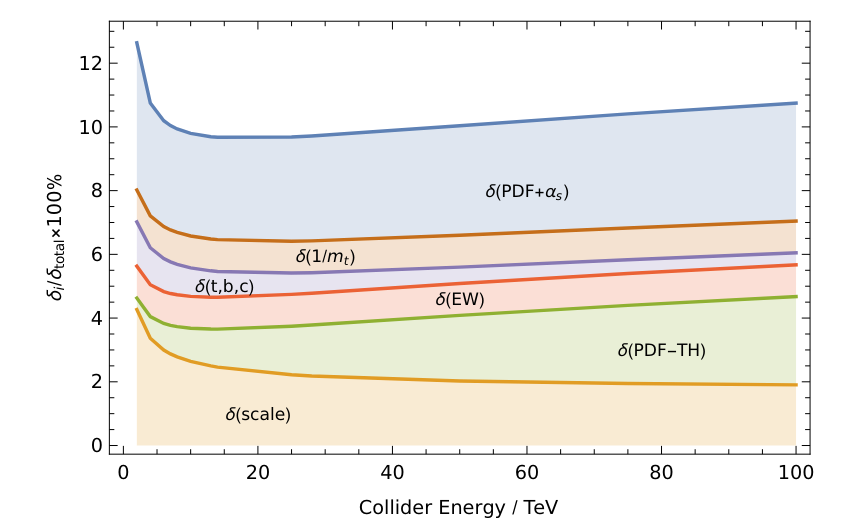
\includegraphics[width=0.99\textwidth]{figures/sources_of_unc_higgs.png}
        \caption*{ \small Uncertainties for inclusive Higgs production \\  {\color{gray}\footnotesize [Dulat, Lazopoulos, Mistleberger, 1802.00827]}}
      \end{figure}

      Since this plot much improvement in:
      \begin{itemize}
        \item NNLO top quark corrections {\color{gray}\footnotesize[Czakon, Harlander, Klappert, Niggetiedt, 2105.04436]}
        \item Mixed QCD-EW corrections {\color{gray}\footnotesize[Becchetti, Bonciani, del Duca, Hirschi, Moriello, Schweitzer, 2010.09451] [Bonetti, Panzer, Smirnov, Tancredi, 2007.09813]}
      \end{itemize}
    \end{column}
  \end{columns}
\end{frame}


\section*{approximate N3LO}
\SectionTitleFrame[\hyperlink{https://arxiv.org/abs/2402.18635}{arXiv: 2402.18635}]


\begin{frame}{Theory requirements for PDFs at N3LO}
  Several theory inputs are needed in a PDF fit:
  \begin{itemize}
    \item Splitting functions for DGLAP evolution
    \item Matching conditions for heavy-quark mass schemes \\
    $ f_i^{\left(n_f+1\right)}=A_{i j} f_j^{\left(n_f\right)} $

    \item DIS coefficient functions
    \item Hadronic cross sections
  \end{itemize}

  \vspace*{2em}
  Not all available at N3LO, but information is available for all. What is the best we can do?
  \begin{itemize}
    \item Use N3LO calculations where known
    \item Construct approximate results where possible
    \item Account for theory uncertainties of the missing or incomplete higher order
  \end{itemize}

  \vspace*{1em}
  No need to wait for complete N3LO results and more information can be included as it becomes available
\end{frame}


\begin{frame}{Splitting functions}
  Complete results for the N3LO splitting functions are not yet available, but some information exists:
  \begin{itemize}
    \item Mellin moments
    \item Small-$x$ limit (threshold resummation)
    \item Large-$x$ limit (BFKL resummation)
    \item Large-$n_f$ limit
  \end{itemize}

  \vspace*{1em}
    \textbf{Idea: combine these limits to construct splitting functions at approximate N3LO}

  \vspace*{1em}
  \only<2>{
    \begin{enumerate}
      \item The approximation is constructed in Mellin space, independently for each order in $n_f$

      $$\gamma_{i j}^{(3)}=\gamma_{i j, n_f}^{(3)}+\gamma_{i j, N \rightarrow \infty}^{(3)}+\gamma_{i j, N \rightarrow 0}^{(3)}+\gamma_{i j, N \rightarrow 1}^{(3)}+\widetilde{\gamma}_{i j}^{(3)}$$

      \item   The remainder term $\widetilde{\gamma}_{i j}^{(3)}$ is constructed as a linear combination of interpolating functions equal to the number of known Mellin moments
      \begin{itemize}
        \item A function for the leading unknown large-N contribution
        \item A function for each of the two leading unknown small-N contribution
        \item 5 functions for the subleading small-N and large-N contributions
      \end{itemize}

      \item The weights of these interpolating functions are determined by equating to the known moments
      \item Then, vary the subleading contributions included in the basis of interpolating functions to estimate incomplete higher order uncertainties (IHOU) on the splitting functions
    \end{enumerate}
  }
\end{frame}


\begin{frame}{Splitting functions}
  \begin{figure}
    \centering
    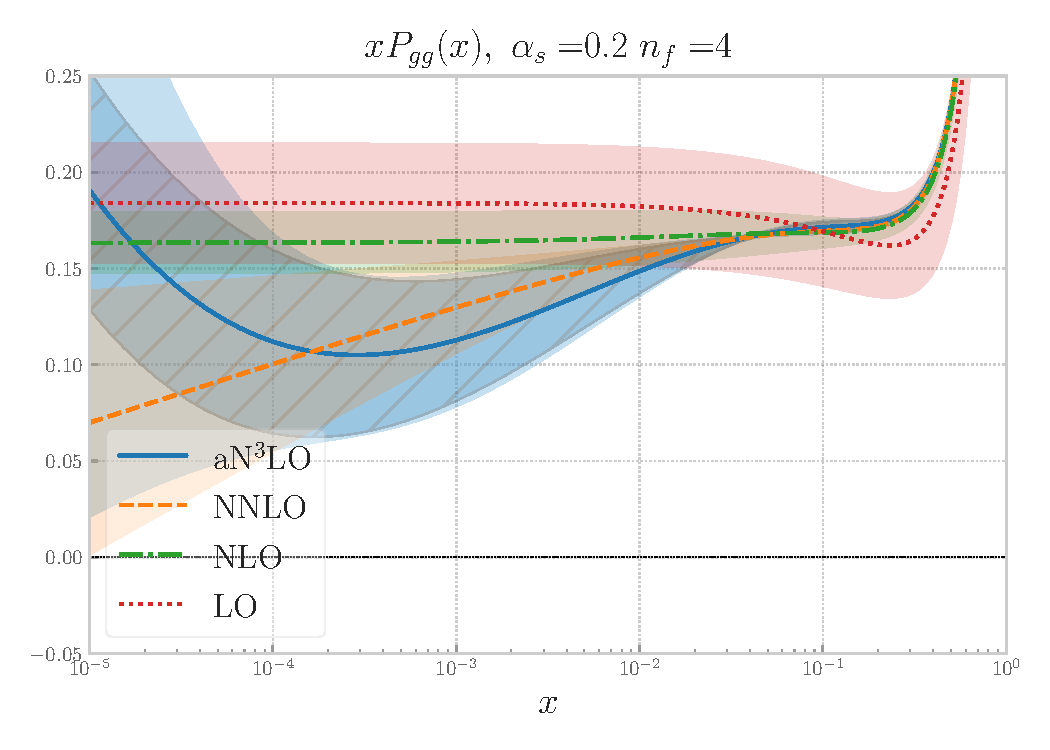
\includegraphics[width=.4\textwidth]{figures/gamma_gg_totu_logx.pdf}
    % 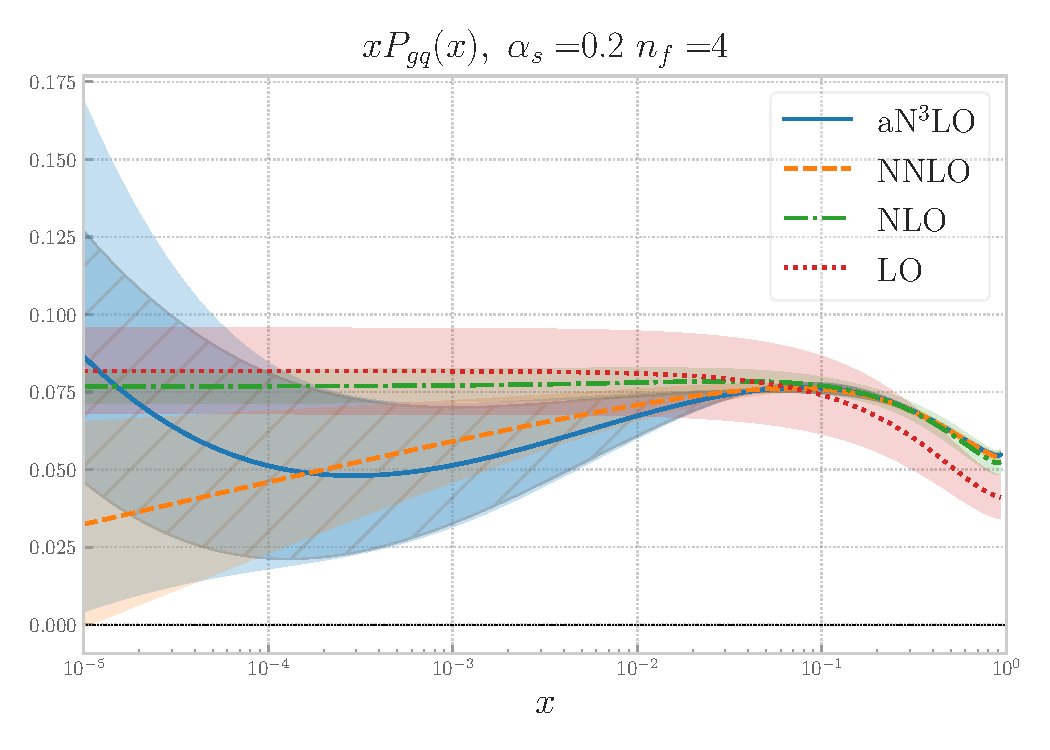
\includegraphics[width=.4\textwidth]{figures/gamma_gq_totu_logx.pdf} \\
    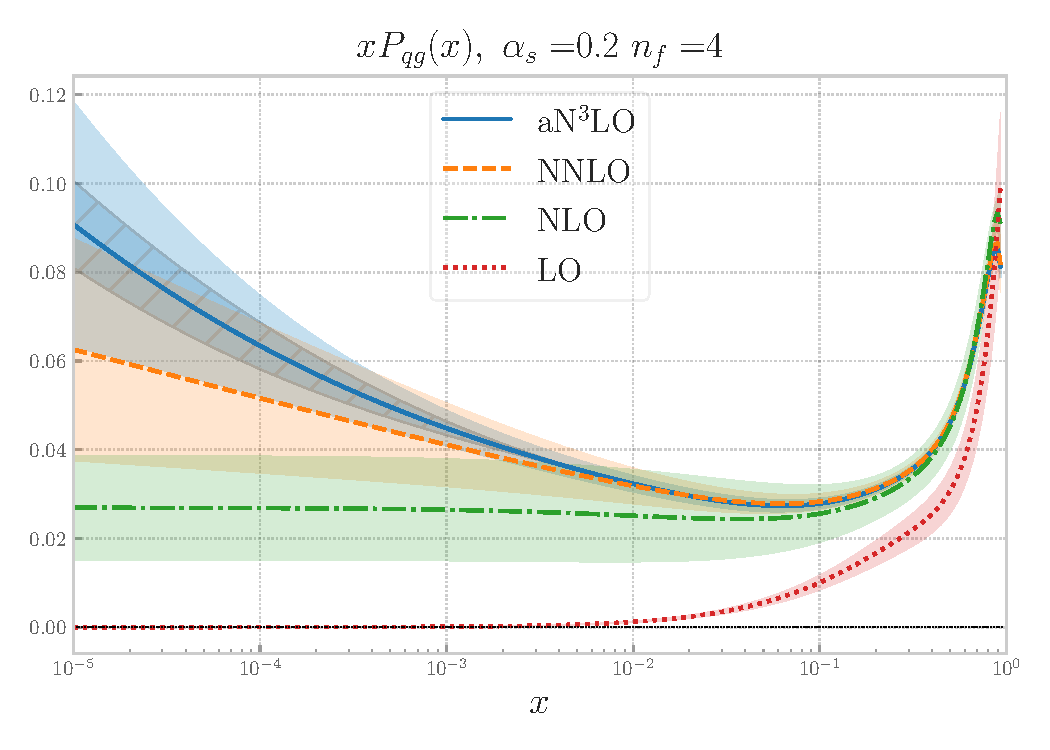
\includegraphics[width=.4\textwidth]{figures/gamma_qg_totu_logx.pdf}
    % 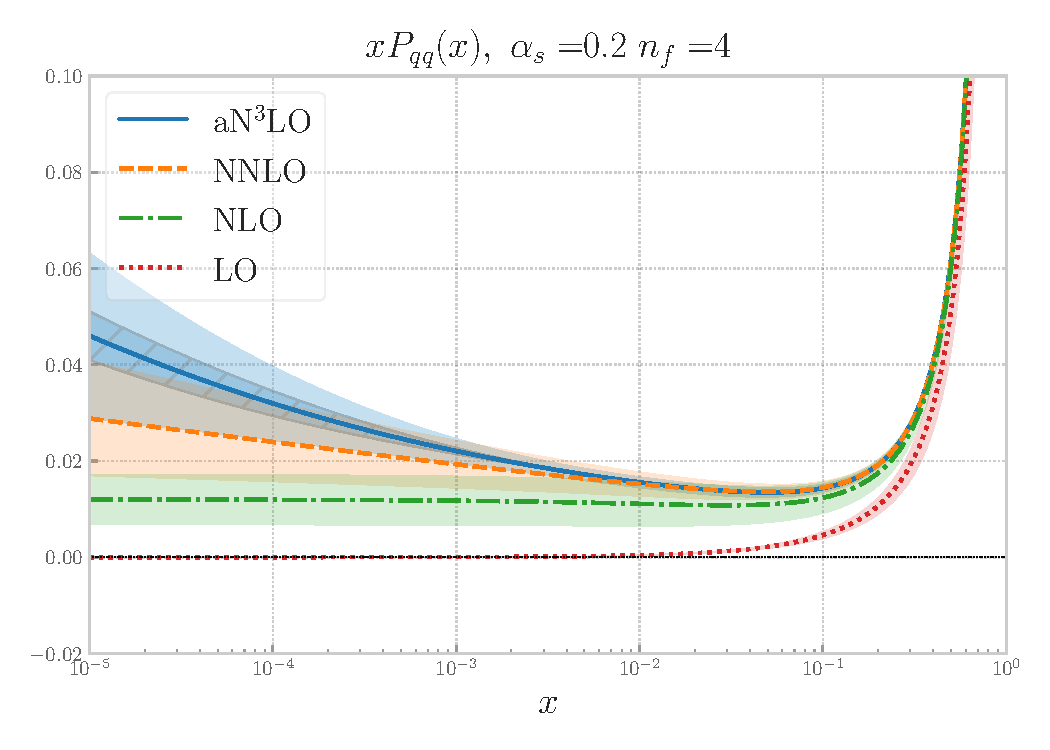
\includegraphics[width=.4\textwidth]{figures/gamma_qq_totu_logx.pdf}
  \end{figure}
  \begin{itemize}
    \item Dark blue band is IHOU only, light blue is sum in quadrature of MHOU and IHOU
    \item Good perturbative agreement at large-$x$
    \item IHOU are not negligible
  \end{itemize}
\end{frame}



\begin{frame}{DGLAP evolution}
  NNPDF4.0 evolved from $Q=1.65$ GeV to $Q=100$ GeV
  \begin{figure}[!t]
    \centering
    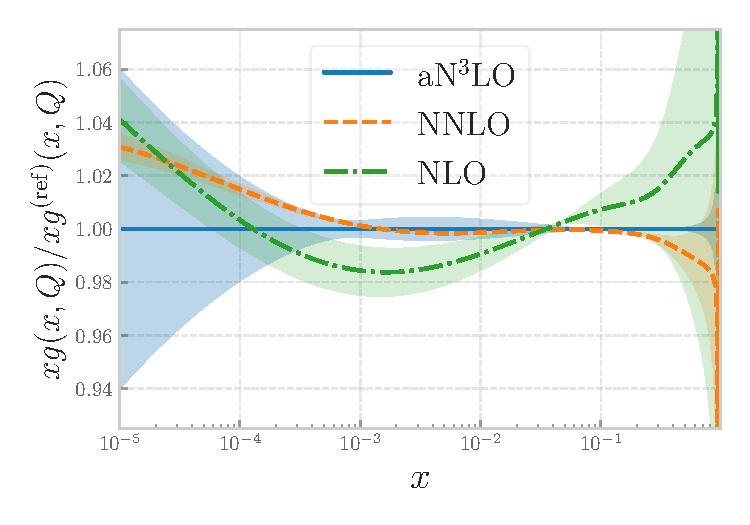
\includegraphics[width=0.4\textwidth]{figures/N3LOevolution-q100gev-ratios_expanded_0.pdf}
    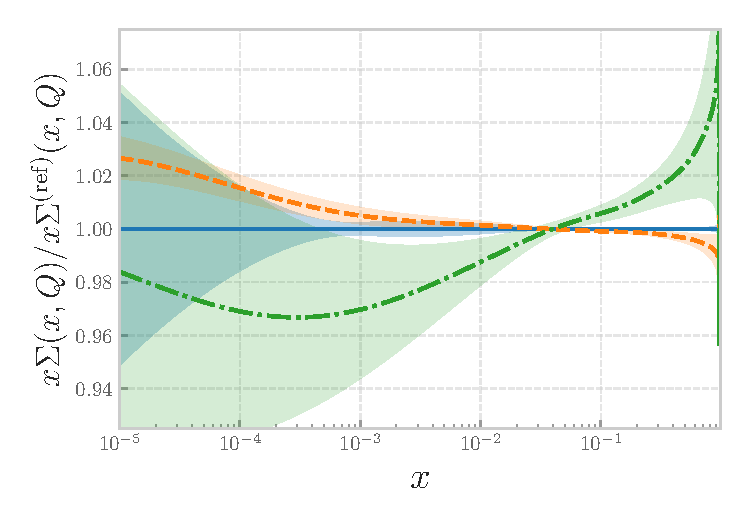
\includegraphics[width=0.4\textwidth]{figures/N3LOevolution-q100gev-ratios_expanded_1.pdf}\\
    % 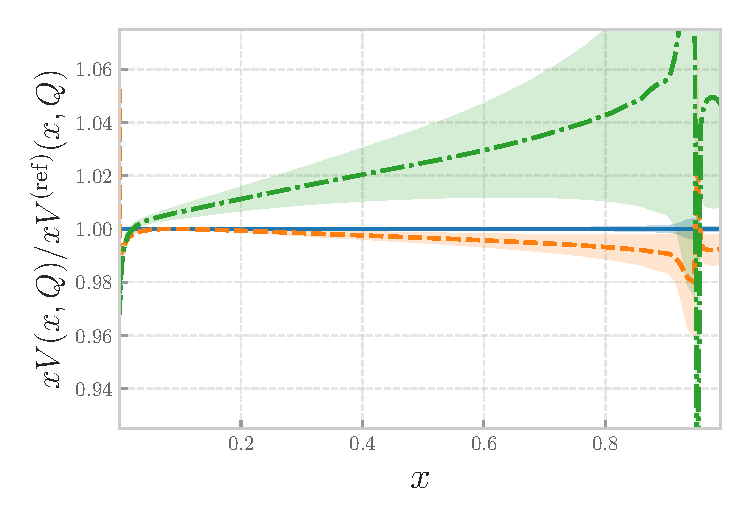
\includegraphics[width=0.49\textwidth]{figures/N3LOevolution-q100gev-ratios_expanded_2.pdf}
    % 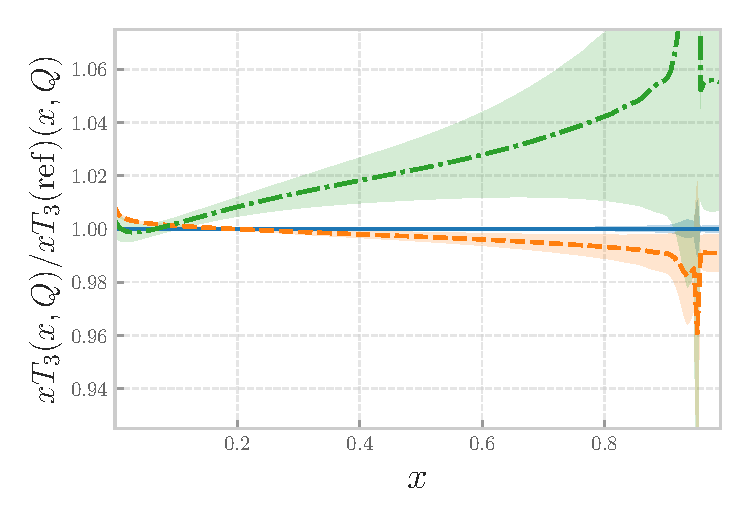
\includegraphics[width=0.49\textwidth]{figures/N3LOevolution-q100gev-ratios_expanded_3.pdf}
  \end{figure}

  \begin{itemize}
    \item Effects of N3LO corrections to DGLAP evolution at most percent level, except at small-$x$ and large-$x$
    \item Good perturbative convergence
  \end{itemize}

\end{frame}

\begin{frame}{DIS coefficient functions}
  \begin{itemize}
    \item DIS coefficient functions are known up to N3LO in the massless limit {\color{gray}\footnotesize [Larin, Nogueira, Van Ritbergen, Vermaseren, 9605317], [Moch Vermaseren Vogt, 0411112, 0504242], [Davies, Moch, Vermaseren, Vogt, 0812.4168, 1606.08907]}
    \item Massive coefficient functions can be constructed by smoothly joining the known limits from threshold and high energy resummation, and the massless limit {\color{gray}\footnotesize [Barontini, Bonvini, Laurenti, in preparation]}
  \end{itemize}

  \vspace*{-0.5em}
  \begin{columns}
    \begin{column}{0.49\textwidth}
      \begin{equation*}
        C^{(3)}(x,m_h^2/Q^2) = C^{(3),{\rm thr}}(x,m_h^2/Q^2) f_1(x) + C^{(3),{\rm asy}}(x,m_h^2/Q^2) f_2(x)
      \end{equation*}
      \begin{align*}
        \begin{split}
          f_1(x) \xrightarrow[x \to x_{\rm max}]{} 1, & \quad  f_2(x) \xrightarrow[x \to x_{\rm max}]{} 0 \\
          f_1(x) \xrightarrow[x \to 0]{} 0, & \quad  f_2(x) \xrightarrow[x \to 0]{} 1
        \end{split}
      \end{align*}
    \end{column}
    \begin{column}{0.49\textwidth}

      \vspace*{2.5em}
      \begin{figure}
        \centering
        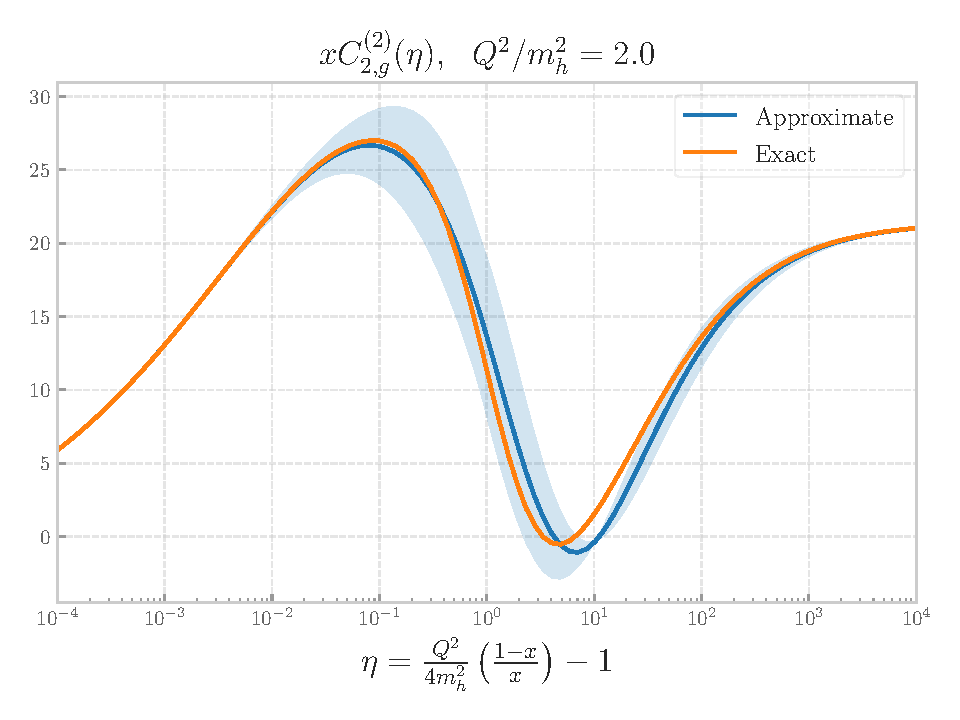
\includegraphics[width=.9\textwidth]{figures/C2g_2_Q2m2_2.0.pdf}
        \caption*{
          Validate the procedure at NNLO \\
          Uncertainty band is obtained by varying interpolation functions
        }
      \end{figure}
    \end{column}
  \end{columns}
\end{frame}


\begin{frame}{Hadronic processes}
  \begin{itemize}
    \item Corrections to collider DY and $W$ production can be included through k-factors
    \item N3LO effects around 1 to 2\% for LHC observables
    \item For many processes N3LO corrections are not available, for those we introduce account for MHOU through $\mu_r$ variations
  \end{itemize}
  \begin{figure}[!t]
    \centering
    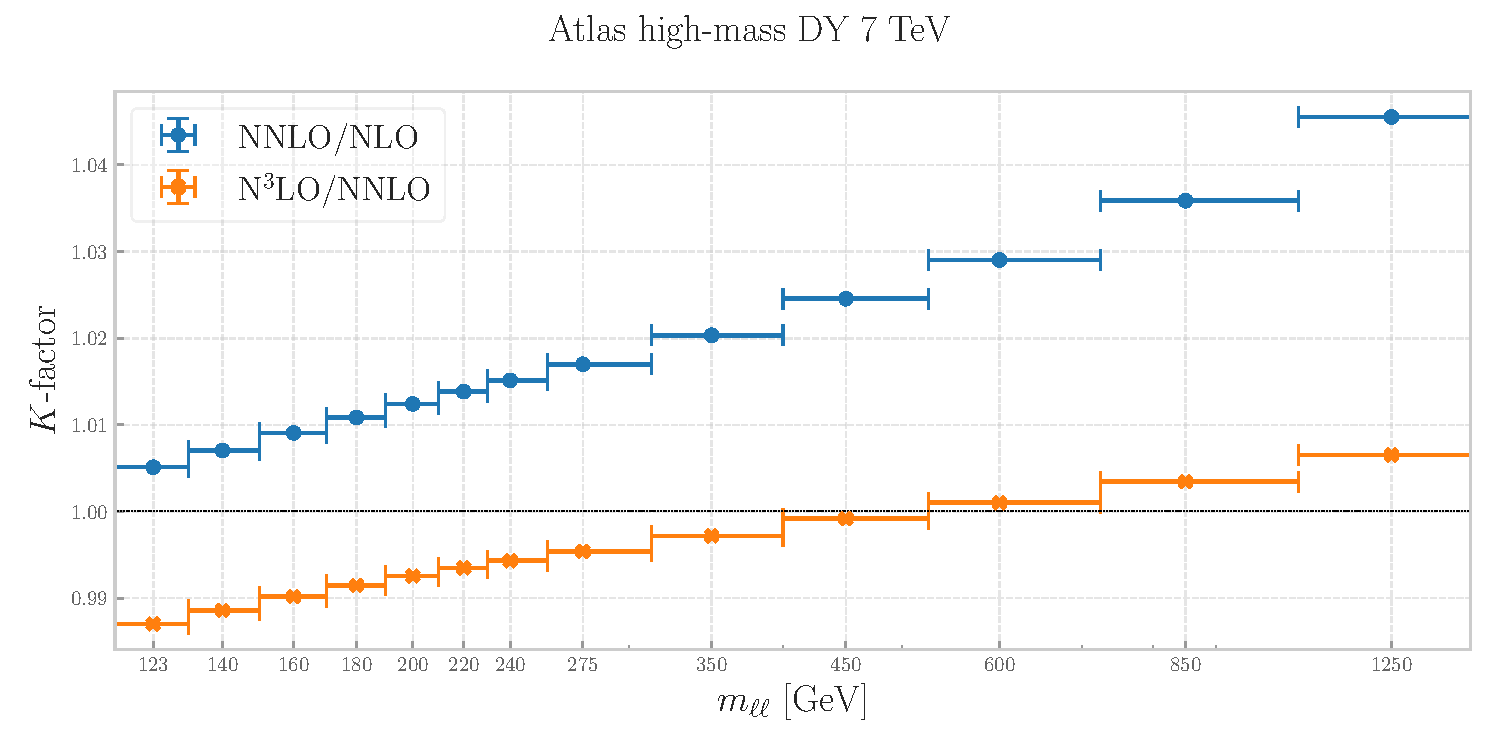
\includegraphics[width=.80\textwidth]{figures/kfactor_ATLASZHIGHMASS49FB.pdf}
  \end{figure}
\end{frame}


\begin{frame}{Theory uncertainties in PDFs}
  \vspace*{1em}
  \begin{itemize}
    \item MHOUs are estimated through 7 point factorization and renormalization scale variations \\
    \begin{figure}
      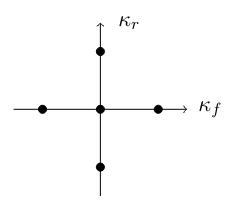
\includegraphics[width=.2\textwidth]{figures/5point.png}
      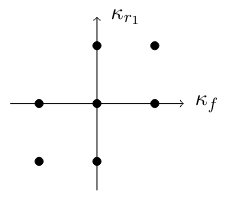
\includegraphics[width=.2\textwidth]{figures/7point.png}
      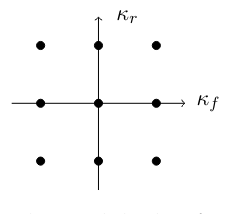
\includegraphics[width=.2\textwidth]{figures/9point.png}
      \caption*{5,7,9 point prescription}
    \end{figure}
    \item In a fit we minimize the $\chi^2$: \\
    $$P(T|D) \propto \exp\left[-\frac{1}{2}\left(T-D\right)C^{-1}\left(T-D\right)\right] = \exp\left[-\frac{1}{2}\chi^2\right]$$
    \item Include theory covmat $C_\mathrm{MHOU}$ at same footing as exp covmat $C = C_\mathrm{exp}+C_\mathrm{MHOU}$ \\
    $$C_{\mathrm{MHOU},ij} = n_{m}\sum_{V_{m}}\left(T_{i}(\kappa_f, \kappa_r) - T_{i}(0, 0)\right)\left(T_{j}(\kappa_f, \kappa_r) - T_{j}(0, 0)\right)$$
    \item Incomplete higher order uncertainties on the approximation of the DGLAP splitting kernels are independent and added in quadrature: \\
    $$C = C_\mathrm{exp}+C_\mathrm{MHOU} + C_\mathrm{IHOU} $$
  \end{itemize}

  \vspace*{1em}
  \only<2>{
    \begin{center}
      Can we trust the faithfulness of these uncertainties on the unknown order?
    \end{center}
  }

\end{frame}


\begin{frame}{Validating the MHOU covmat}
  \textbf{Validate the MHOU procedure} by comparing the NLO covmat with estimated MHOUs to the known NNLO-NLO shifts
  \begin{figure}[!t]
    \centering
      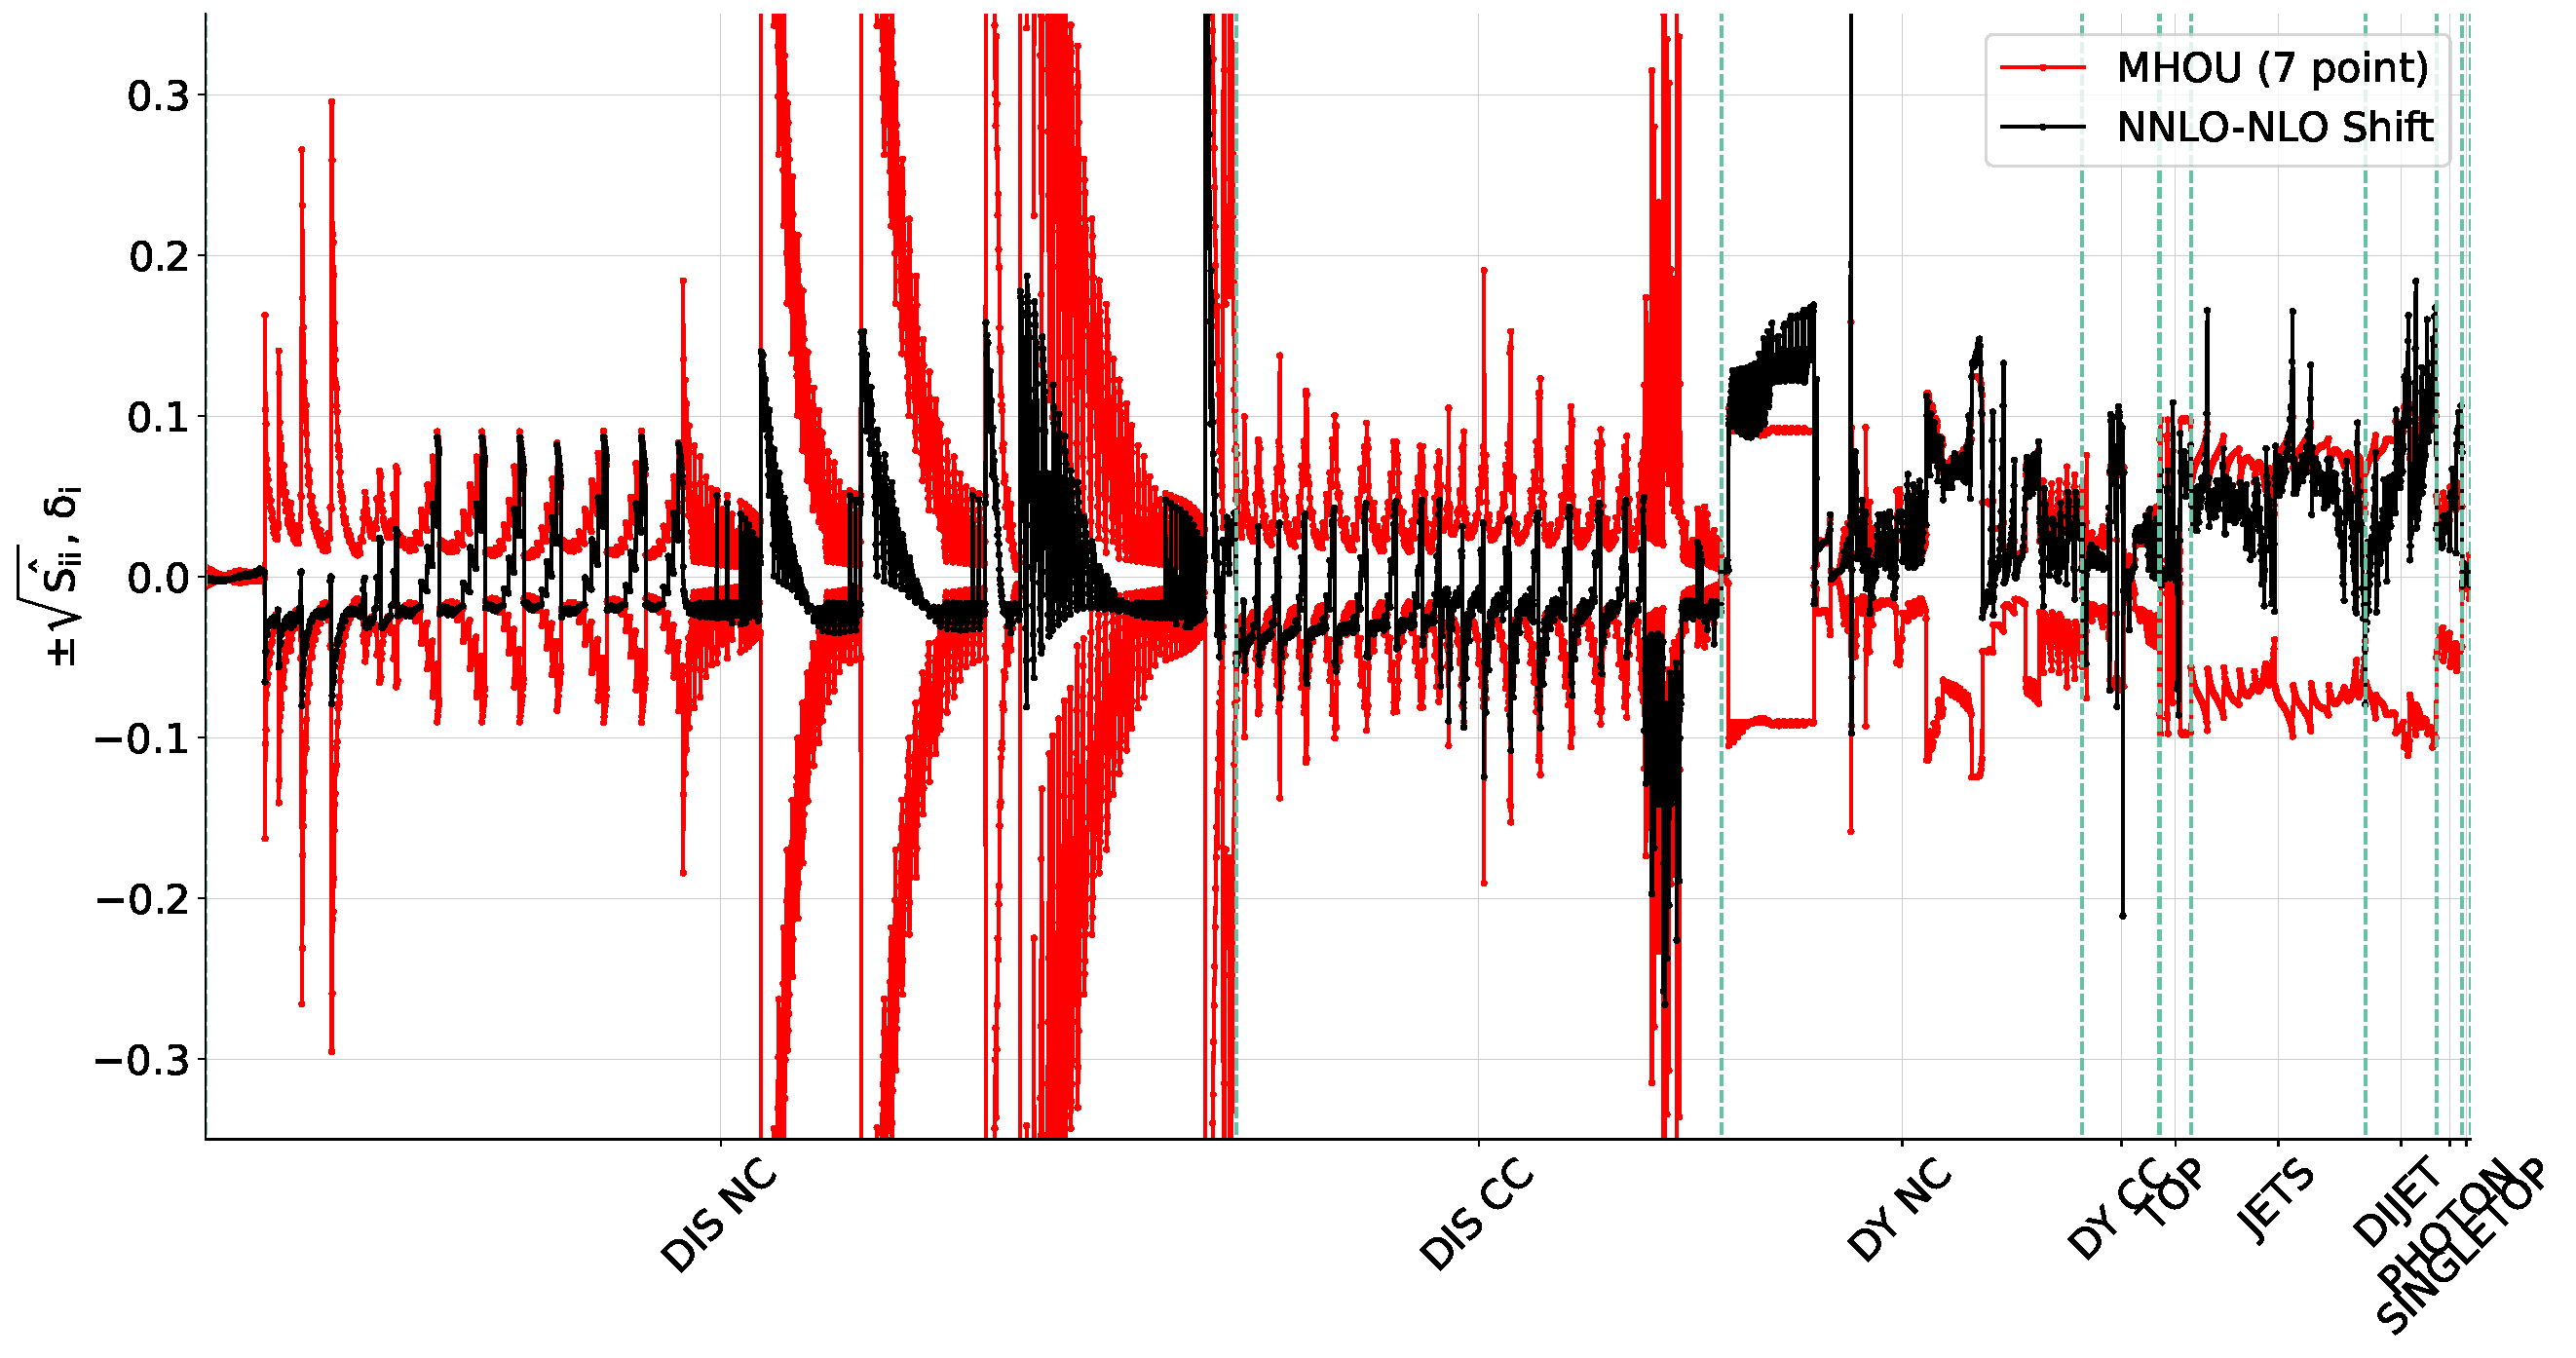
\includegraphics[width=0.8\textwidth]{figures/shift_validation.pdf}
  \end{figure}
\end{frame}


\begin{frame}{Fit quality}
  \begin{figure}[!t]
    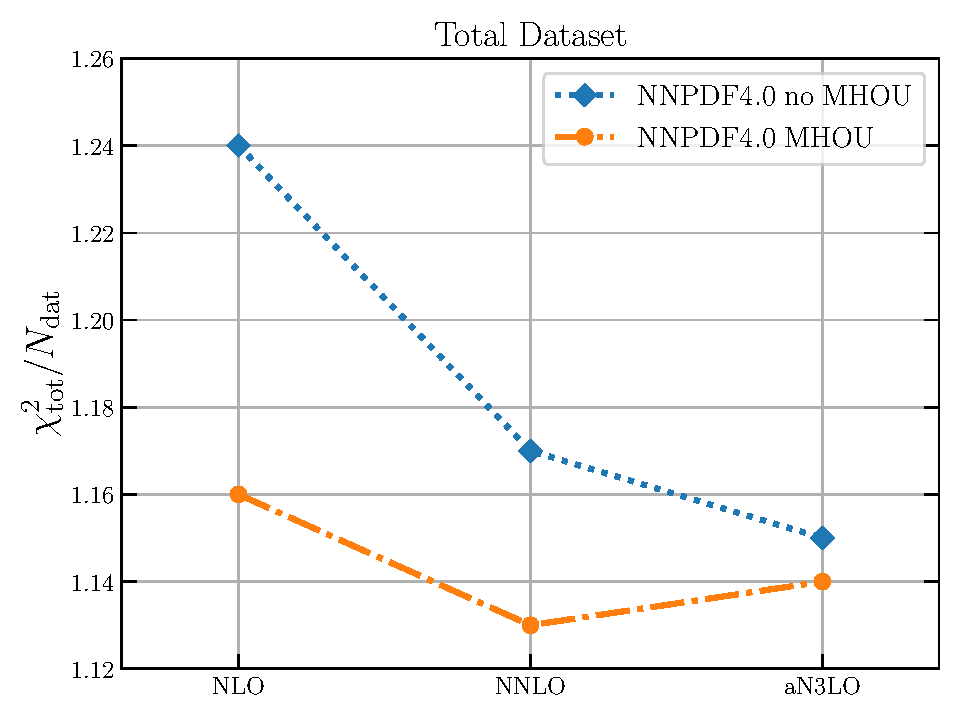
\includegraphics[width=.4\textwidth]{figures/chi2_n3lo_summary.pdf}
  \end{figure}
  \begin{itemize}
    \item Without MHOUs the $\chi^2$ improves with the perturbative accuracy
    \item With MHOUs the $\chi^2$ stabilizes significantly
    \item At N3LO MHOUs have a small impact on the $\chi^2$
  \end{itemize}
\end{frame}

\begin{frame}{Higgs production}
  \begin{figure}[!t]
    \centering
    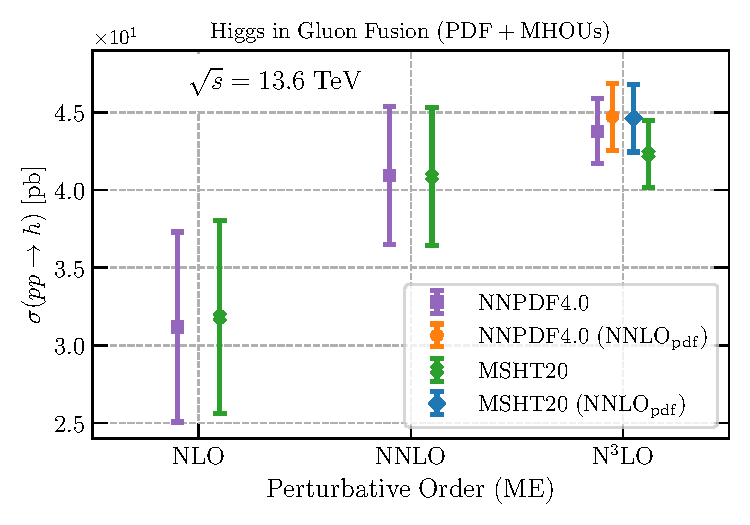
\includegraphics[width=0.49\linewidth]{figures/higgs-ggF-n3lo.pdf}
    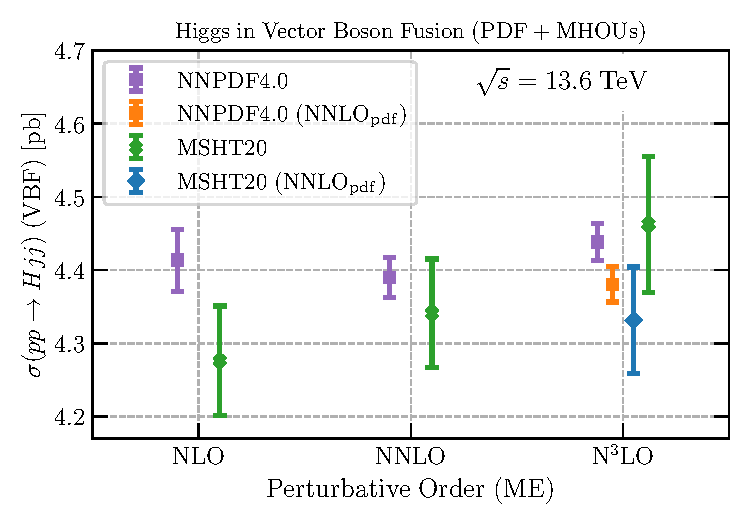
\includegraphics[width=0.49\linewidth]{figures/H_VBF-n3lo.pdf}
  \end{figure}
  \begin{itemize}
    \item Matrix elements for both Higgs in gluon fusion and VBF available at N3LO
    \item N3LO correction to Higgs in gluon fusion, small suppression compared to NNLO PDF (purple vs orange)
    \item Higgs in VBF perturbatively stable
  \end{itemize}
\end{frame}


\begin{frame}{Drell-Yan}
  \begin{figure}[!t]
    \centering
    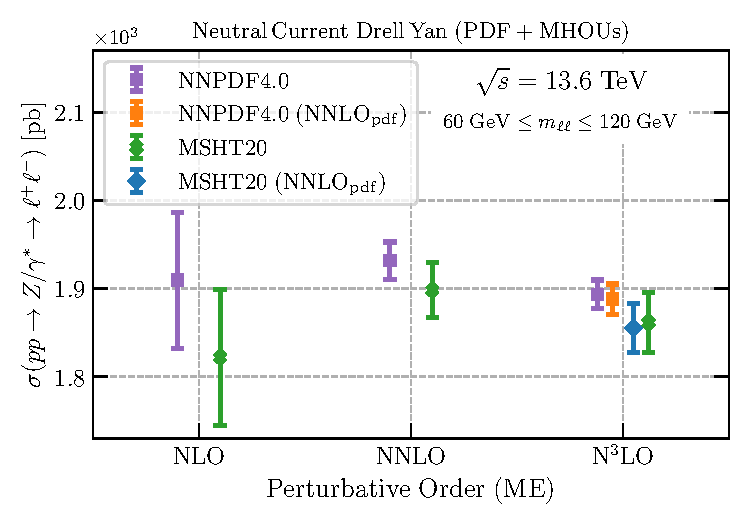
\includegraphics[width=0.49\linewidth]{figures/Z_60_120-n3lo.pdf}
    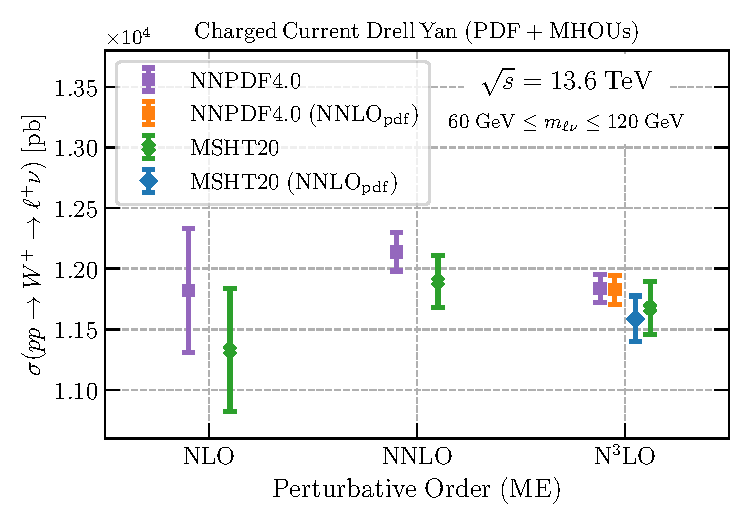
\includegraphics[width=0.49\linewidth]{figures/Wp_60_120-n3lo.pdf}
  \end{figure}
  \begin{itemize}
    \item Good convergence also for quark initiated processes
  \end{itemize}
\end{frame}




\section*{QED}
\SectionTitleFrame[\hyperlink{https://arxiv.org/abs/2401.08749}{arXiv: 2401.08749}]


\begin{frame}{A QED PDF set}
  The QED PDF set extends the NNLO QCD PDF in two ways:
  \begin{itemize}
    \item Add a photon PDF since processes can be sensitive to photon initiated channels \\
    The momenum sumrule is modified accordingly:
    \begin{equation*}
      \int_0^1 dx\, x \left(  \Sigma(x) + g(x) + \gamma(x) \right) =1
    \end{equation*}


    \item Modify the DGLAP running to account for photon radiation: \\
    $P=P_{QCD}(\alpha_s) + P_{QCD\otimes QED}(\alpha_s,\alpha)$\\
  \end{itemize}

  \begin{figure}
    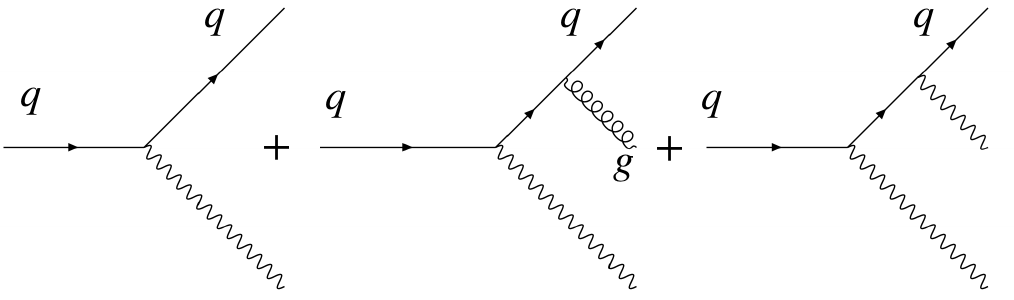
\includegraphics[width=0.6\textwidth]{qed_splitting.png}
    \caption*{$P_{QCD\otimes QED}=\alpha P^{(0,1)}+\alpha \alpha_s P^{(1,1)}+\alpha^2 P^{(0,2)}$}
  \end{figure}

    % \begin{column}{0.49\textwidth}
    %   \begin{figure}
    %     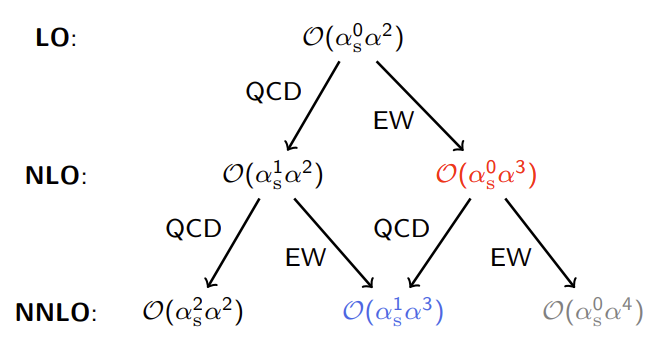
\includegraphics[width=0.99\textwidth]{figures/ewcorrections_dy.png}
    %     \caption*{Example: EW corrections in DY\\ {\color{gray}\footnotesize [C. Schwan DIS 2021]}}
    %   \end{figure}
    % \end{column}
\end{frame}


\begin{frame}{The photon PDF}
  \begin{columns}
    \begin{column}{0.59\textwidth}
      \begin{itemize}
        \item Data does not provide strong constraints on the photon so fitting is not optimal

        \item The photon PDF can be computed from DIS structure functions using the luxQED result {\color{gray}\footnotesize[Manohar, Nason, Salam, Zanderighi, 1607.04266, 1708.01256]}
        \begin{equation*}
          \begin{split}
            & x \gamma(x, \mu^2)
            =
            \frac{2}{\alpha (\mu^2)} \int\limits_x^1 \frac{dz}{z}
            \Biggl\{ \int_{m_p^2x^2 \over 1-z}^{\mu^2 \over 1-z} \frac{dQ^2}{Q^2}
            \alpha^2(Q^2) \Biggl[ -z^2 F_L(x/z, Q^2) \\
            & + \left( z P_{\gamma q}(z) + \frac{2 x^2 m_p^2}{Q^2} \right)
            F_2(x/z, Q^2)\Biggr] - \alpha^2(\mu^2) z^2 F_2(x/z, \mu^2)\Biggr\}
          \end{split}
        \end{equation*}

        \item An iterative procedure  is used to address the interplay between the photon and other PDFs due to the momentum sumrule
        \begin{equation*}
          \int_0^1 dx\, x \left( \Sigma(x) + g(x) + \gamma(x) \right) =1
        \end{equation*}
      \end{itemize}
    \end{column}

    \begin{column}{0.39\textwidth}
      \vspace*{-1.5em}
      \begin{figure}
        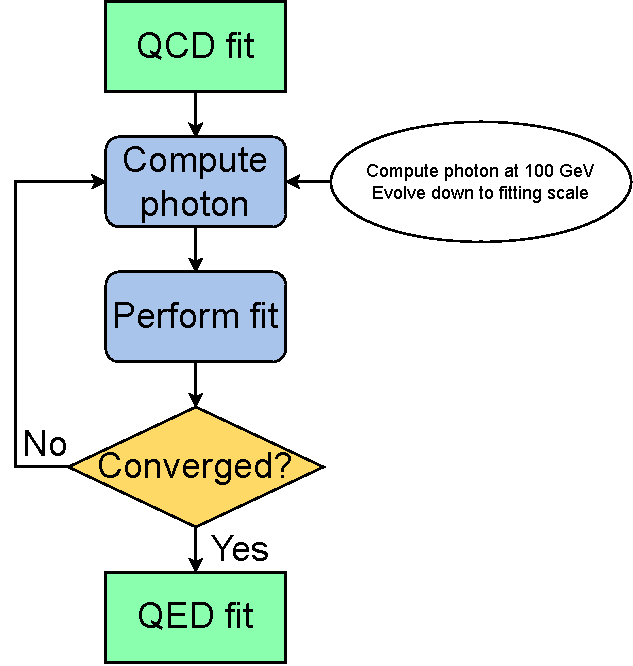
\includegraphics[width=0.9\textwidth]{figures/luxqed_iteration.pdf}
        \caption*{\color{gray}\footnotesize [NNPDF3.1QED: 1712.07053]}
      \end{figure}
    \end{column}
  \end{columns}

\end{frame}


\begin{frame}{Impact of the photon on other PDFs}

  \begin{figure}[!t]
    \centering
    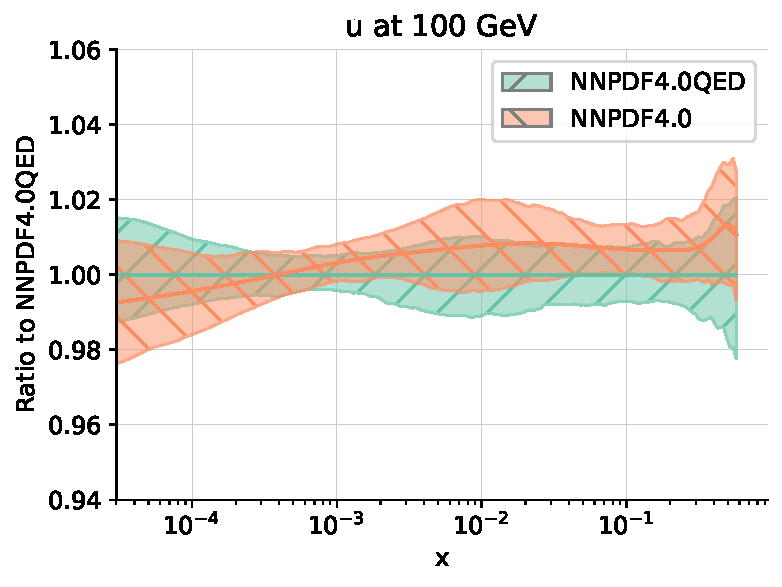
\includegraphics[width=.49\textwidth]{figures/plot_pdfs_u_qed.pdf}
    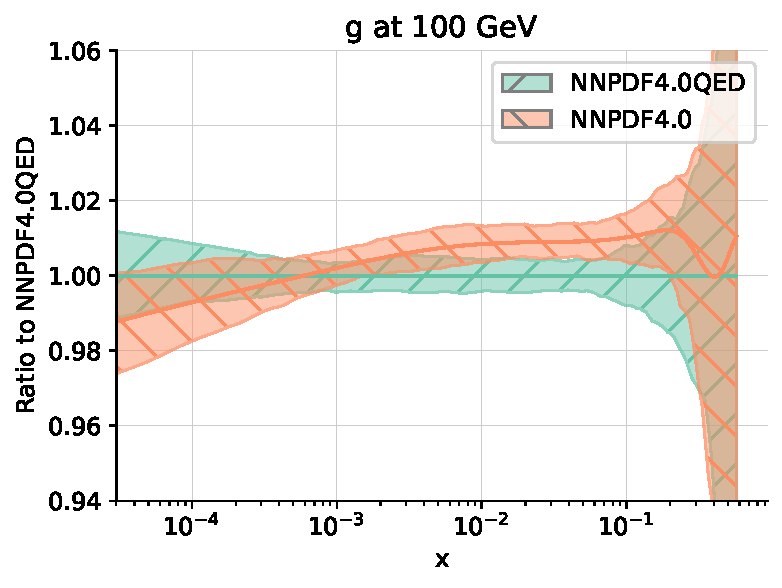
\includegraphics[width=.49\textwidth]{figures/plot_pdfs_g_qed.pdf}\\
  \end{figure}

  \begin{itemize}
    \item Non-negligible impact, but PDFs are in agreement within uncertainty
    \item Gluon reduced due to momentum sum rule with photon carrying additional momentum
  \end{itemize}
\end{frame}


% \begin{frame}{Results: photon PDF and luminosity}
%   \begin{center}
%     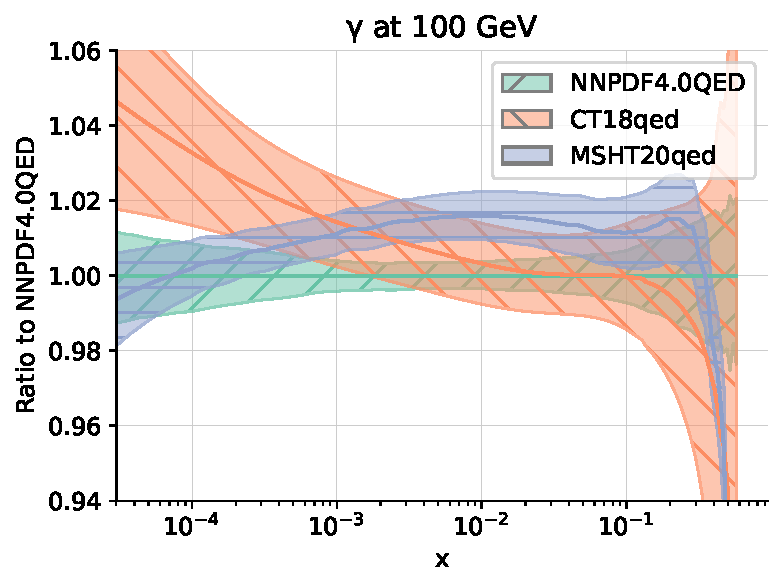
\includegraphics[width=0.3\textwidth]{figures/photon_comparison.pdf}
%     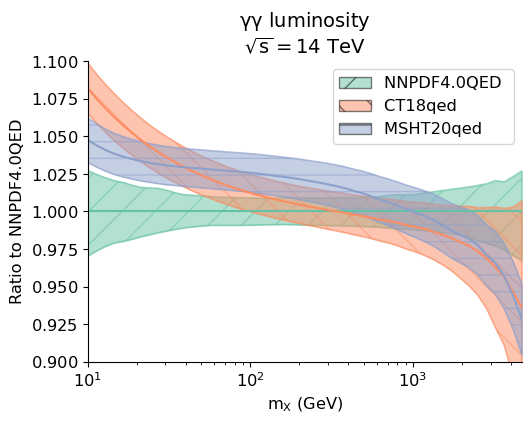
\includegraphics[width=0.3\textwidth]{figures/pp_lumi_comparison.png}
%     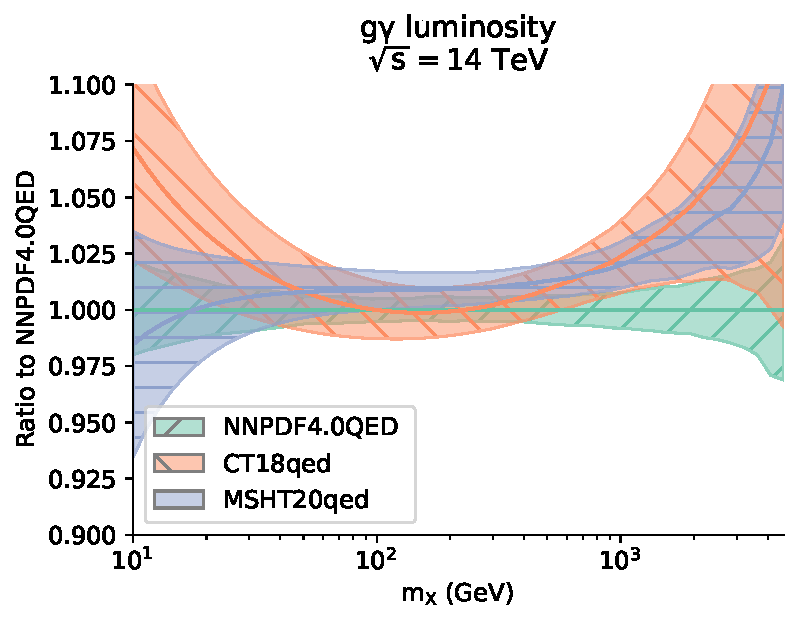
\includegraphics[width=0.3\textwidth]{figures/gp_lumi_comparison.pdf}
%   \end{center}
%   \begin{itemize}
%     \item Because all groups use the luxQED formalism, the photon PDFs agree at percent level
%     \item Luminosity generally in agreement, but differ at very small and very large invariant mass
%   \end{itemize}
% \end{frame}


\begin{frame}{Phenomenological impact}
  \begin{columns}[T]
    \begin{column}{0.49\textwidth}
      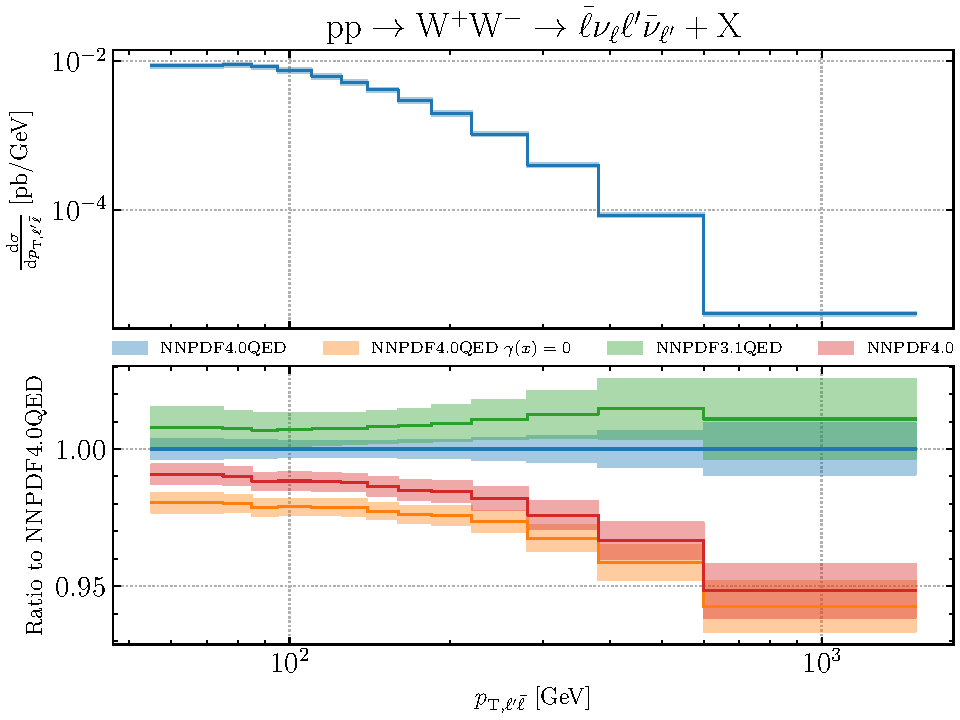
\includegraphics[width=0.9\textwidth]{figures/NNPDF_WPWM_14TEV_40_PHENO-internal.pdf}
    \end{column}
    \begin{column}{0.49\textwidth}
      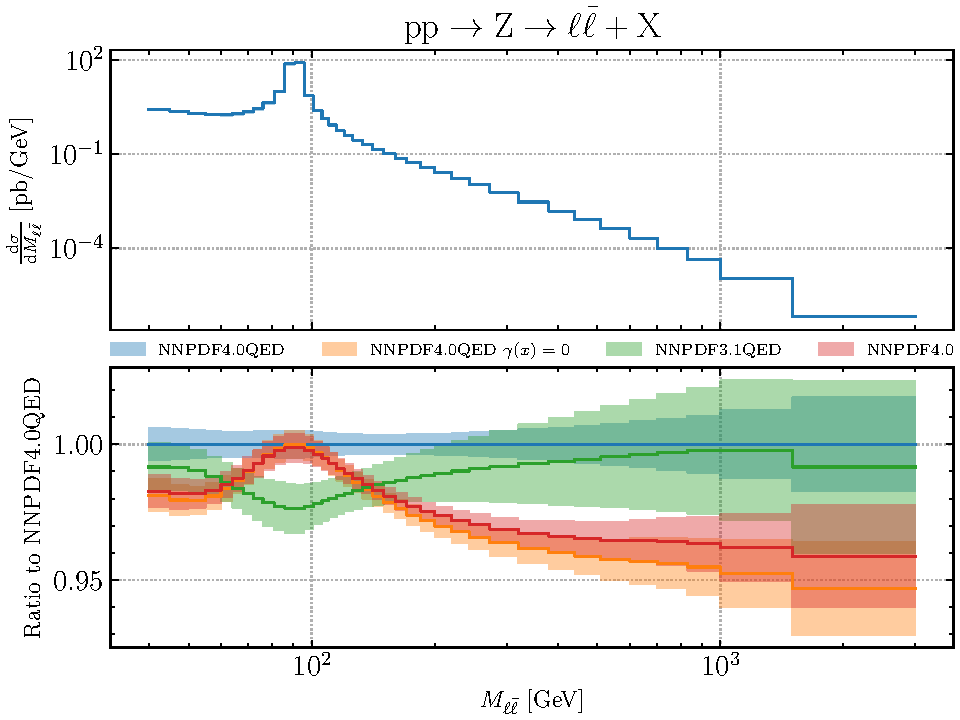
\includegraphics[width=0.9\textwidth]{figures/NNPDF_DY_14TEV_40_PHENO-internal.pdf}
    \end{column}
  \end{columns}

  \vspace*{1em}
  \begin{itemize}
    % \item NLO in both QCD and QED, only PDF uncertainties are shown
    \item Photon induced effects are up to 5\% in the large invariant mass and large-$p_T$ region (blue vs orange)
    \item The QED corrections to the quarks and gluon are at most 1\% (red vs orange)
  \end{itemize}
\end{frame}


\section*{$\alpha_s$ from NNPDF4.0}
\SectionTitleFrame[In preparation]



\begin{frame}{Correlations between $\alpha_s$ and the PDFs}
  \begin{columns}[T]
    \begin{column}{0.49\textwidth}
      \begin{itemize}
        \item Usually $\alpha_s$ determination is done by repeating a PDF fit at different values of $\alpha_s$ and performing a parabolic fit
      \end{itemize}
    \end{column}
    \begin{column}{0.49\textwidth}
      \only<1>{
      \begin{figure}
        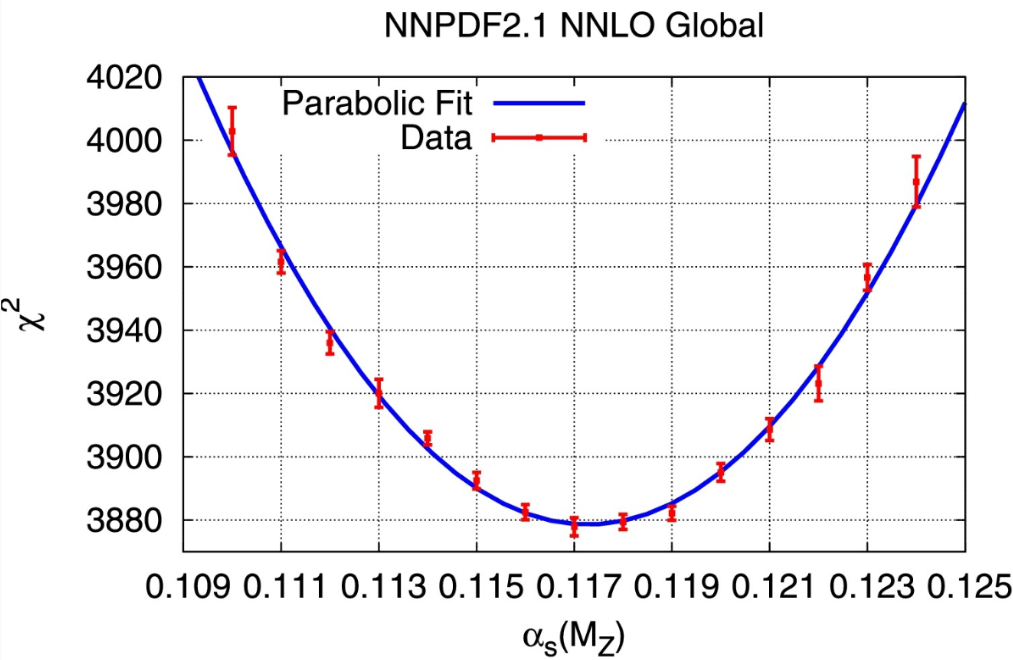
\includegraphics[width=0.7\textwidth]{exp_method.png}
        \caption*{\color{gray}\footnotesize \hyperlink{https://arxiv.org/pdf/1110.2483}{NNPDF, 1110.2483}}
      \end{figure}
      }
    \end{column}
  \end{columns}
\end{frame}

\begin{frame}{Correlations between $\alpha_s$ and the PDFs}
  \begin{columns}[T]
    \begin{column}{0.49\textwidth}
      \begin{itemize}
        \item Usually $\alpha_s$ determination is done by repeating a PDF fit at different values of $\alpha_s$ and performing a parabolic fit
        \item Such a determination misses correlations between $\alpha_s$ and the PDF parameters $\theta$, leading to \textbf{underestimated uncertainties}
      \end{itemize}
    \end{column}
    \begin{column}{0.49\textwidth}
      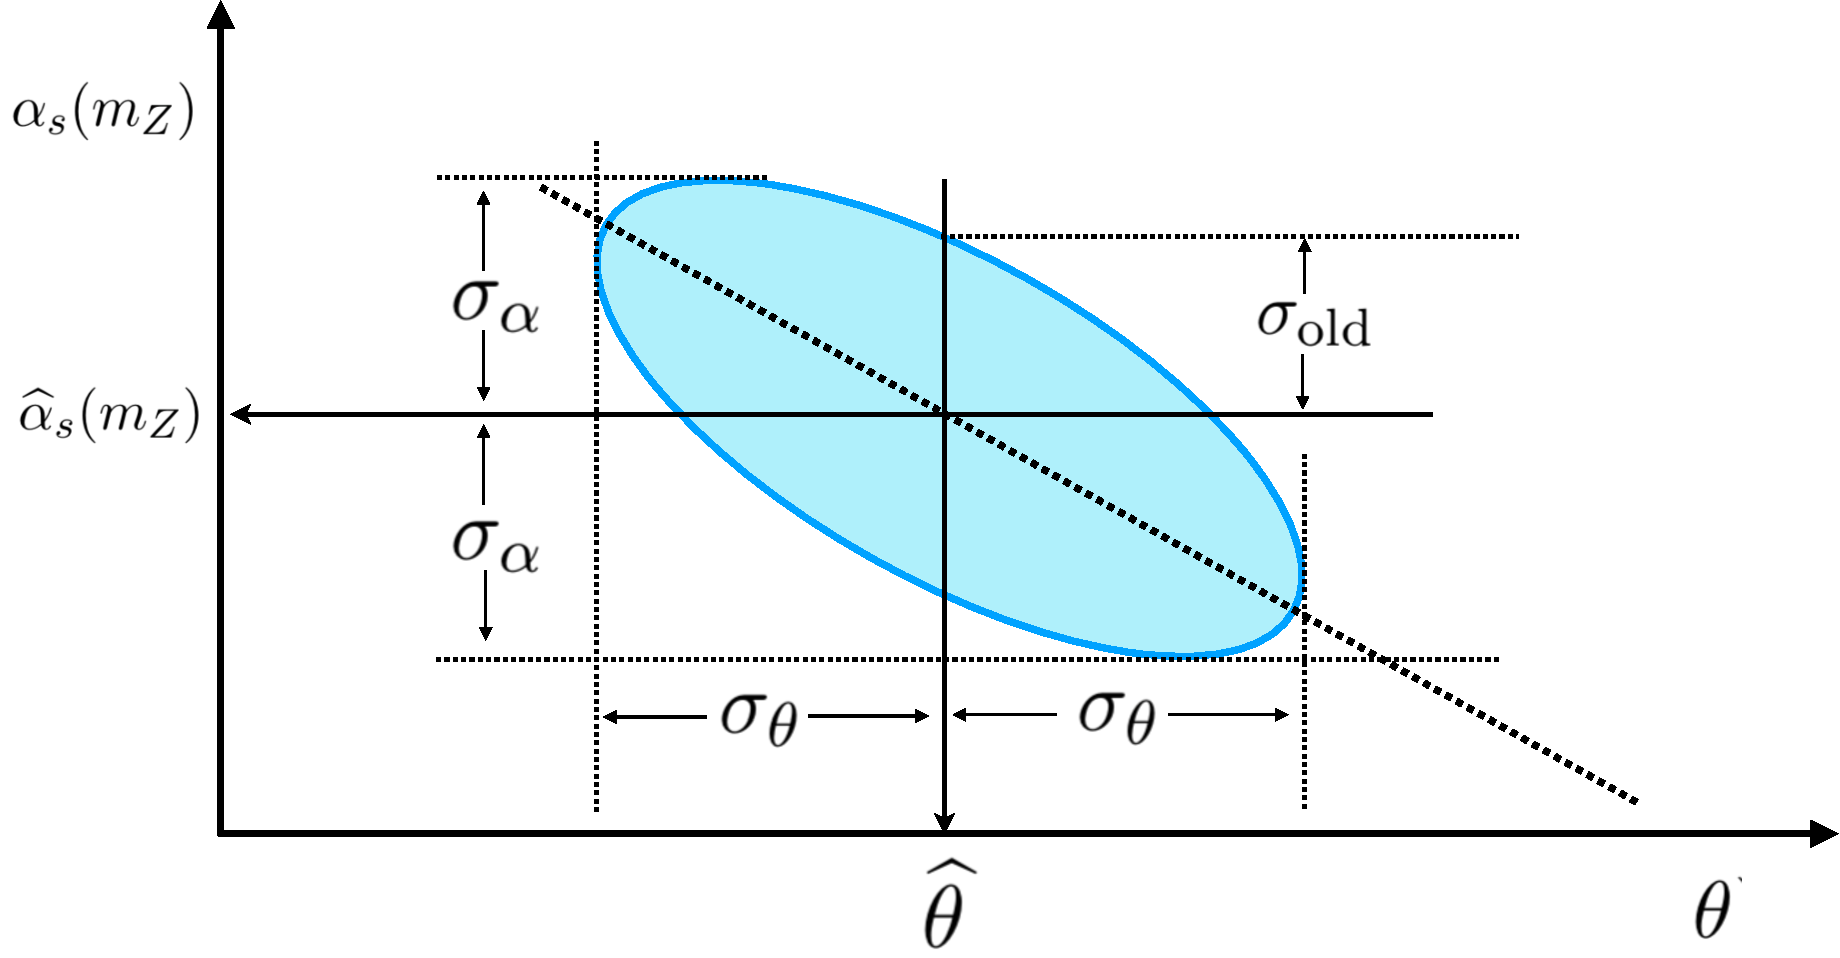
\includegraphics[width=0.9\textwidth]{ellipse.pdf}
    \end{column}
  \end{columns}
\end{frame}

\begin{frame}{Propagating uncertainties in NNPDF}

  Data is fully defined by central values $\mu_i$ and covariance matrix $\operatorname{cov}_{ij}$
  \begin{enumerate}
    \item Produce a Monte Carlo sample of data replicas
    \item Perform a PDF fit to each replica
    \item[$\Rightarrow$] PDF replicas now encode experimental uncertainties!
  \end{enumerate}

  \vspace*{2em}
  \begin{center}
    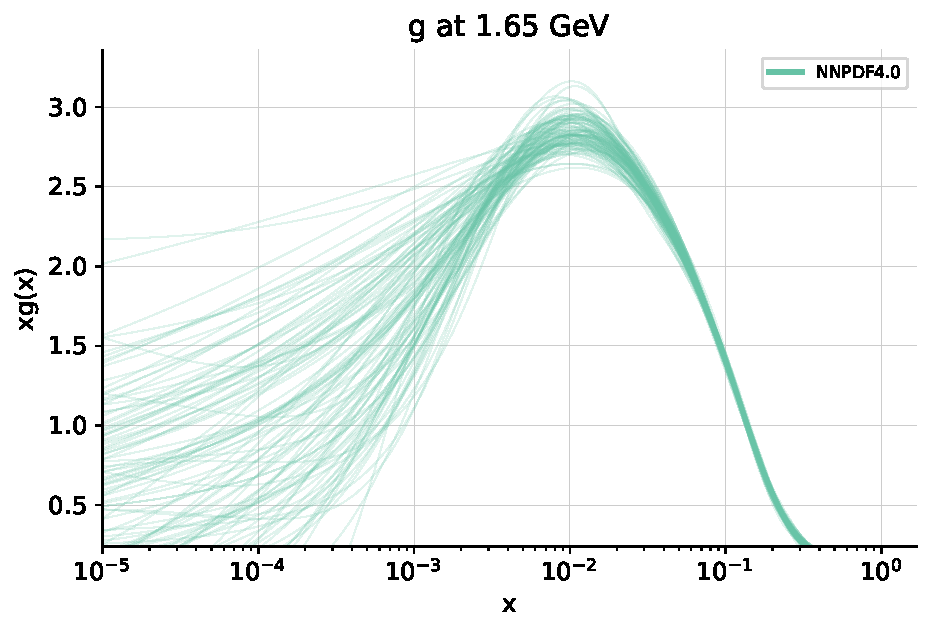
\includegraphics[width=0.4\textwidth]{replicas_g.pdf}
    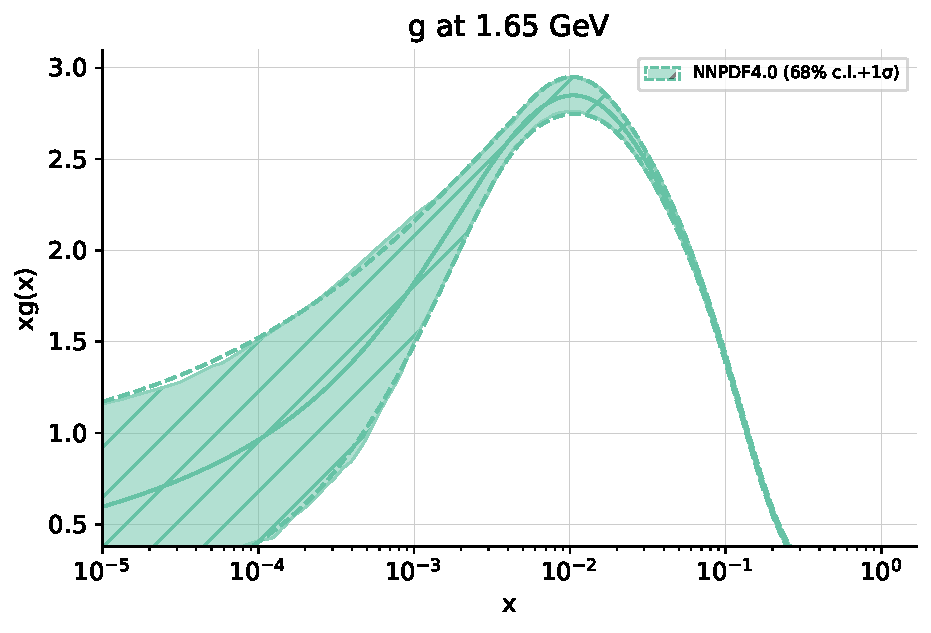
\includegraphics[width=0.4\textwidth]{band_g.pdf}
  \end{center}
\end{frame}


\begin{frame}{A simultaneous optimization of $\alpha_s$}
  Ideally we would minimize simultaneously $\alpha_s$ and the PDF parameters but due to theories being stored in pre-computed grids at fixed values of $\alpha_s$ this is impractical

  % A simultaneous minimization implies solving the system of coupled equations
  % \begin{align}
  %   \label{eq:partial_theta}
  %   \frac{\partial}{\partial \theta} \chi^2(\alpha_s, \theta) &= 0 \\
  %   \frac{\partial}{\partial \alpha_s} \chi^2(\alpha_s, \theta) &= 0
  % \end{align}

  \vspace*{1em}

  A possible way to find the minimum in ($\alpha_s, \theta$) space is:
  \begin{enumerate}
    \item generate a set of pseudodata replicas
    \item fit these data replicas for different values of $\alpha_s$ (thus finding minima for $\theta$)
    \item for each replica, fit a parabola to get a $\chi^2(\alpha_s)$ profile
    \item each minimum corresponds to a sampled $\alpha_s$ value
  \end{enumerate}


  \begin{figure}
    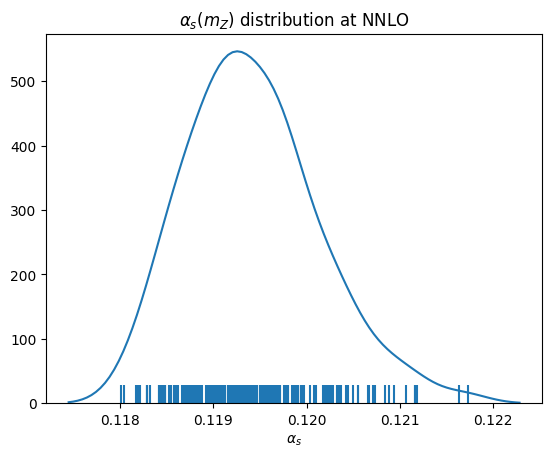
\includegraphics[width=0.5\textwidth]{alphas_density.png}
  \end{figure}

\end{frame}


\begin{frame}{$\alpha_s$ from correlated theory uncertainties}

  % Remember, in a PDF fit we minimize $\chi^2$:\\
  % $P(T|D) \propto \exp\left[-\frac{1}{2}\left(T-D\right)^T\mathrm{Cov}^{-1}\left(T-D\right)\right]
  % = \exp\left[-\frac{1}{2}\chi^2\right]$

  We can also determine $\alpha_s$ in a Bayesian way from a nuisance parameter

  \begin{itemize}
    \item Model theory uncertainty as a correlated shift: \\
    $T \rightarrow T + \lambda \beta $, \quad $\beta=\frac{\partial}{\partial \alpha_s}T$ ($\beta$ is constructed form discrete shifts)\\
    ${\color{red}P(T|D,\lambda) }\propto \exp\left[-\frac{1}{2}\left(T+\lambda\beta-D\right)^T\mathrm{Cov}_\mathrm{exp}^{-1}\left(T+\lambda\beta-D\right)\right]$

    \item Choose a unit-width Gaussian prior\\
    ${\color{blue} P(\lambda)} \propto \exp\left[-\frac{1}{2}\lambda^2\right]$

    \item Marginalizing over $\lambda$ to get  ${\color{green} P(T|D)}$ \\
    % ${\color{green} P(T|D)} \propto \int d\lambda \exp\left[Z^{-1}\left(\lambda-\bar{\lambda}\right)^2\right] \exp\left[-\frac{1}{2}\left(T-D\right)^T\left(\mathrm{Cov}_\mathrm{exp}+\beta\beta^T\right)^{-1}\left(T-D\right)\right] \propto \exp\left[\chi^2\right]$  \\

  \end{itemize}

  We thus have all the ingredients to compute the posterior for the parameter encoding a shift in $\alpha_s$: \\
  $$P(\lambda|T,D) = \frac{{\color{red}P(T|D,\lambda) }{\color{blue} P(\lambda)}}{{\color{green} P(T|D)}} \propto \exp\left[-\frac{1}{2}Z^{-1}(\lambda - \bar{\lambda})\right]$$
  for some functions $0<Z<1$ and $\bar{\lambda}$.

  \vspace{1em}
  \begin{center}
    The prior for $\alpha_s$ can be updated by the addition of new information!
  \end{center}


  \vspace*{1em}
  {\color{gray} \footnotesize Ball, Pearson, \hyperlink{https://arxiv.org/abs/2105.05114}{2105.05114}}

  % \vfill
  % \textbf{Idea:}
  % \begin{enumerate}
  %   \item Construct a (prior) $\alpha_s$ theory covariance matrix from variations around a fixed value of $\alpha_s$
  %   \item Include this covariance matrix in a fit
  %   \item Compute the posterior distribution of $\alpha_s$
  % \end{enumerate}
\end{frame}


\begin{frame}{Validating the methodology}
  We use ``closure tests'' to validate our methodology:
  \begin{enumerate}
    \item Take a given value of $\alpha_s$
    \item Make theoretical predictions for all data
    \item Generate data replicas distributed according to the covariance matrix
    \item Perform the usual fits and analysis
    \item Test statistics on these ``simulated experimental samplings''
    \begin{itemize}
      \item Is the chosen value of $\alpha_s$ within 1$\sigma$ for 68\% of cases?
    \end{itemize}
  \end{enumerate}

  \vspace{1em}
  Preliminary results suggests the “correlated replicas” method \textbf{faithfully determines $\alpha_s$}!

  \vspace{1em}
  A test of the theory uncertainties method is ongoing
\end{frame}


\begin{frame}{PRELIMINARY NNPDF4.0 results at NNLO}
  Only \textbf{PDF uncertainty:}
  \begin{itemize}
    \item NNPDF3.1 result (2018): $\alpha_s(m_Z) = 0.1185 \pm 0.0005$
    \item NNPDF3.1-like dataset: $\alpha_s(m_Z) = 0.1185 \pm 0.0006$
    \item[$\Rightarrow$] Perfect agreement between NNPDF4.0 and NNPDF3.1 methodologies!
    \item NNPDF4.0 dataset: $\alpha_s(m_Z) = 0.1204 \pm 0.0004$
  \end{itemize}

  \vspace*{1em}
  \textbf{PDF uncertainty + MHOU:}
  \begin{itemize}
    \item NNPDF4.0 dataset: $\alpha_s(m_Z)=0.1194 \pm 0.0007$
    \item NNPDF3.1 dataset: $\alpha_s(m_Z) = 0.1182 \pm 0.0008$
  \end{itemize}

  \vspace*{1em}
  \textbf{LHC data seems to prefer a larger value of $\alpha_s$}

  \vspace*{1em}
  Other sources of uncertainty that need to be studied:
  \begin{itemize}
    \item Methodological (e.g. is there dependence on $f$ for $\chi^2(f(\alpha_s))$?)
    \item Higher twist
    \item Nuclear corrections
  \end{itemize}

  \vspace*{3em}
  \begin{center}
    Finally, \textbf{extend up to aN3LO}
  \end{center}

\end{frame}


\section{Summary and outlook}

\begin{frame}[c]{Summary and outlook}
  \begin{itemize}\setlength{\itemsep}{30pt}
    \item N3LO PDFs and QED corrections are a requirement for LHC predictions at 1\% accuracy
    \item Good perturbative convergence is observed, and NNLO and aN3LO agree with uncertainties
    \item A PDF determination at aN3LO QCD and NLO QED to appear soon
    \item An $\alpha_s$ determination at aN3LO with estimated MHOU and validated methodologies is underway
  \end{itemize}

  \vspace*{7em}
  \only<2>{
  \begin{center}
      {\Large \textbf{Thank you for your attention!}}
  \end{center}
  }
\end{frame}



\appendix
\section{Backup}


\begin{frame}{Determination of the photon PDF}
  \begin{columns}[T]
    \begin{column}{0.59\textwidth}
      Initially the photon PDF has been determined in different ways:
      \begin{itemize}
        \item physical model: sensitive to underlying model
        \item fitting: data does not provide strong constraints
      \end{itemize}

      \vspace*{0.5em}
      However with the LUXqed approach it can be computed perturbatively \\
      based on the observation that the heavy-lepton production cross-section can be written in two ways:
      \begin{itemize}
        \item in terms of structure functions $F_2$, $F_L$
        \item in terms of PDFs (including the photon)
      \end{itemize}

      \vspace*{0.5em}
      luxQED result {\color{gray}\small[Manohar, Nason, Salam, Zanderighi: 1607.04266, 1708.01256]}:
      \vspace*{-0.8em}
      \begin{equation*}
        \begin{split}
          & x \gamma(x, \mu^2)
          =
          \frac{2}{\alpha (\mu^2)} \int\limits_x^1 \frac{dz}{z}
          \Biggl\{ \int_{m_p^2x^2 \over 1-z}^{\mu^2 \over 1-z} \frac{dQ^2}{Q^2}
          \alpha^2(Q^2) \Biggl[ -z^2 F_L(x/z, Q^2) \\
          & + \left( z P_{\gamma q}(z) + \frac{2 x^2 m_p^2}{Q^2} \right)
          F_2(x/z, Q^2)\Biggr] - \alpha^2(\mu^2) z^2 F_2(x/z, \mu^2)\Biggr\}
        \end{split}
      \end{equation*}
    \end{column}

    \begin{column}{0.39\textwidth}
      \vspace*{-2.5em}
      \begin{figure}
        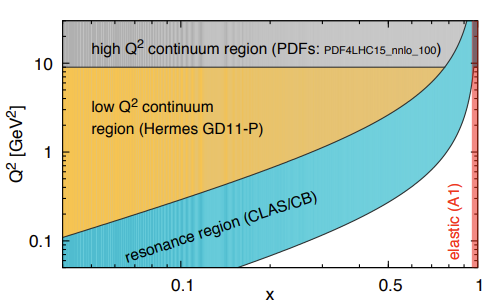
\includegraphics[width=0.89\textwidth]{figures/dataluxqed.png}
        \caption*{Input to construct $F_2$ and $F_L$}
        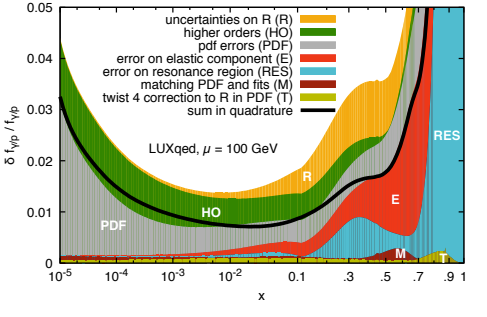
\includegraphics[width=0.89\textwidth]{figures/luxQED_uncs.png}
        \caption*{Sources of uncertainty}
      \end{figure}
    \end{column}
  \end{columns}
\end{frame}


\begin{frame}{LUXqed PDF determinations}
  LUXqed has been used in all of the most recent QED PDFs:
  \begin{itemize}
      \item LUXqed\_plus\_PDF4LHC15 {\color{gray}\small [1607.04266]}
      \item LUXqed17\_plus\_PDF4LHC15 {\color{gray}\small [1708.01256]}
      \item MMHT2015qed {\color{gray}\small [1907.02750]}
      \item NNPDF3.1luxQED {\color{gray}\small [1712.07053]}
      \item CT18lux and CT18qed {\color{gray}\small [2106.10299]}
      \item MSHT20QED {\color{gray}\small [2111.05357]}
      \item MSHT20qed\_an3lo {\color{gray}\small [2312.07665]}
      \item NNPDF4.0QED {\color{gray}\small [2401.08749 ]}
  \end{itemize}
\end{frame}

% \begin{frame}{Results: photon PDF and luminosity}
%   \begin{center}
%     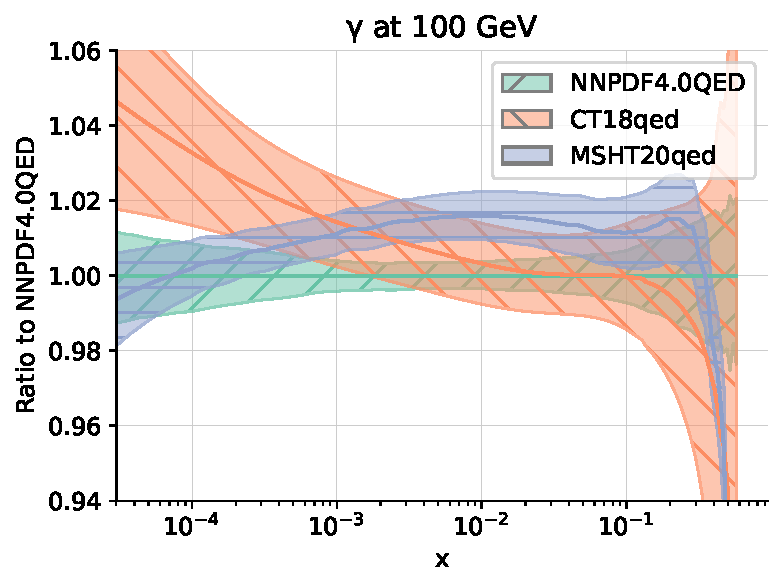
\includegraphics[width=0.3\textwidth]{figures/photon_comparison.pdf}
%     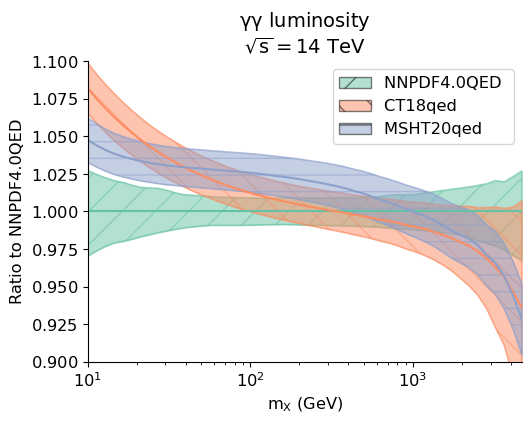
\includegraphics[width=0.3\textwidth]{figures/pp_lumi_comparison.png}
%     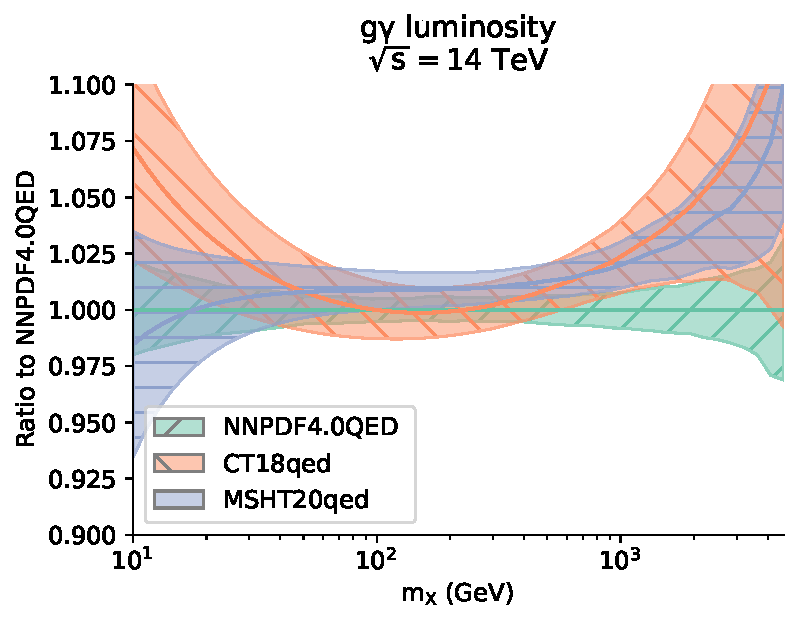
\includegraphics[width=0.3\textwidth]{figures/gp_lumi_comparison.pdf}
%   \end{center}
%   \begin{itemize}
%     \item Because all groups use the luxQED formalism, the photon PDFs agree at percent level
%     \item Luminosity generally in agreement, but differ at very small and very large invariant mass
%   \end{itemize}
% \end{frame}


% ============================================================================


\begin{frame}{Incomplete higher order uncertainties covmat}
  \begin{itemize}
    \item We construct an IHOU matrix following a similar approach by varying the subleading functions
    \item IHOU are independent of MHOU so the uncertainties are added in quadrature
    $$C = C_\mathrm{exp}+C_\mathrm{MHOU}+C_\mathrm{IHOU}$$
  \end{itemize}

  \begin{columns}
    \begin{column}{0.49\textwidth}
      \begin{figure}[!t]
        \centering
        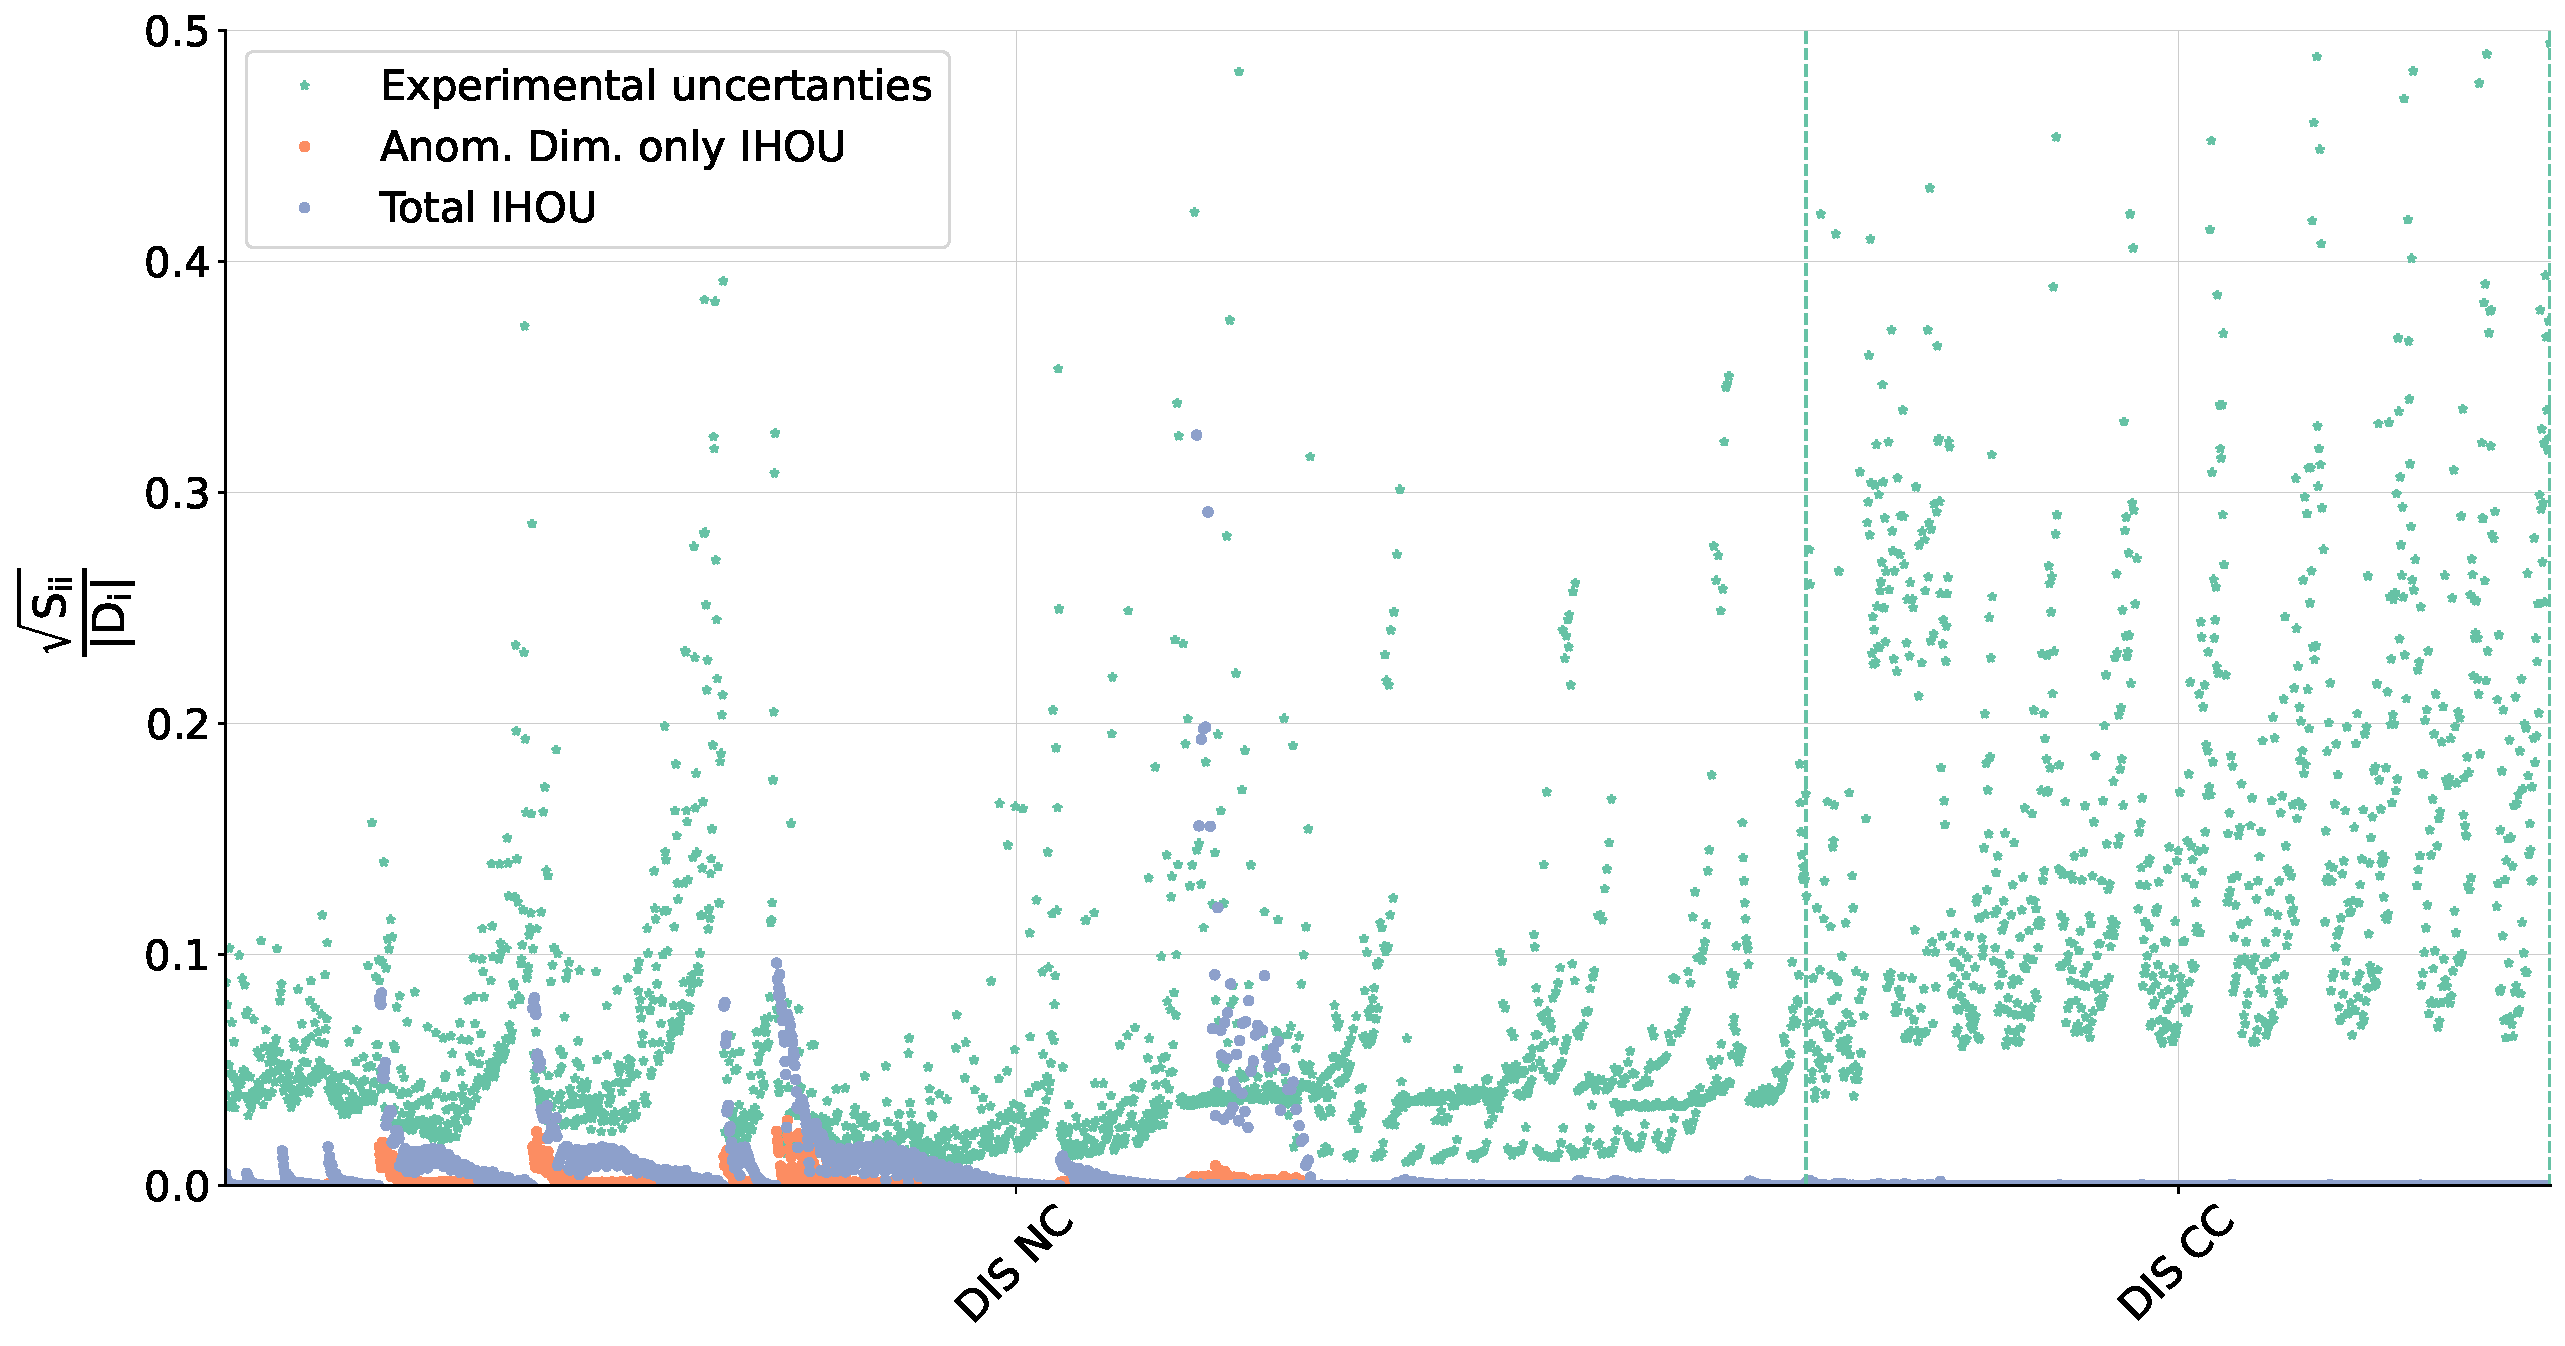
\includegraphics[width=.9\textwidth]{figures/diag_cov_dis_ihou.pdf}
        \caption*{IHOU have a large effect on small-$x$, low-$Q$ DIS data
        }
      \end{figure}
    \end{column}
    \begin{column}{0.49\textwidth}
      \begin{figure}[!t]
        \centering
        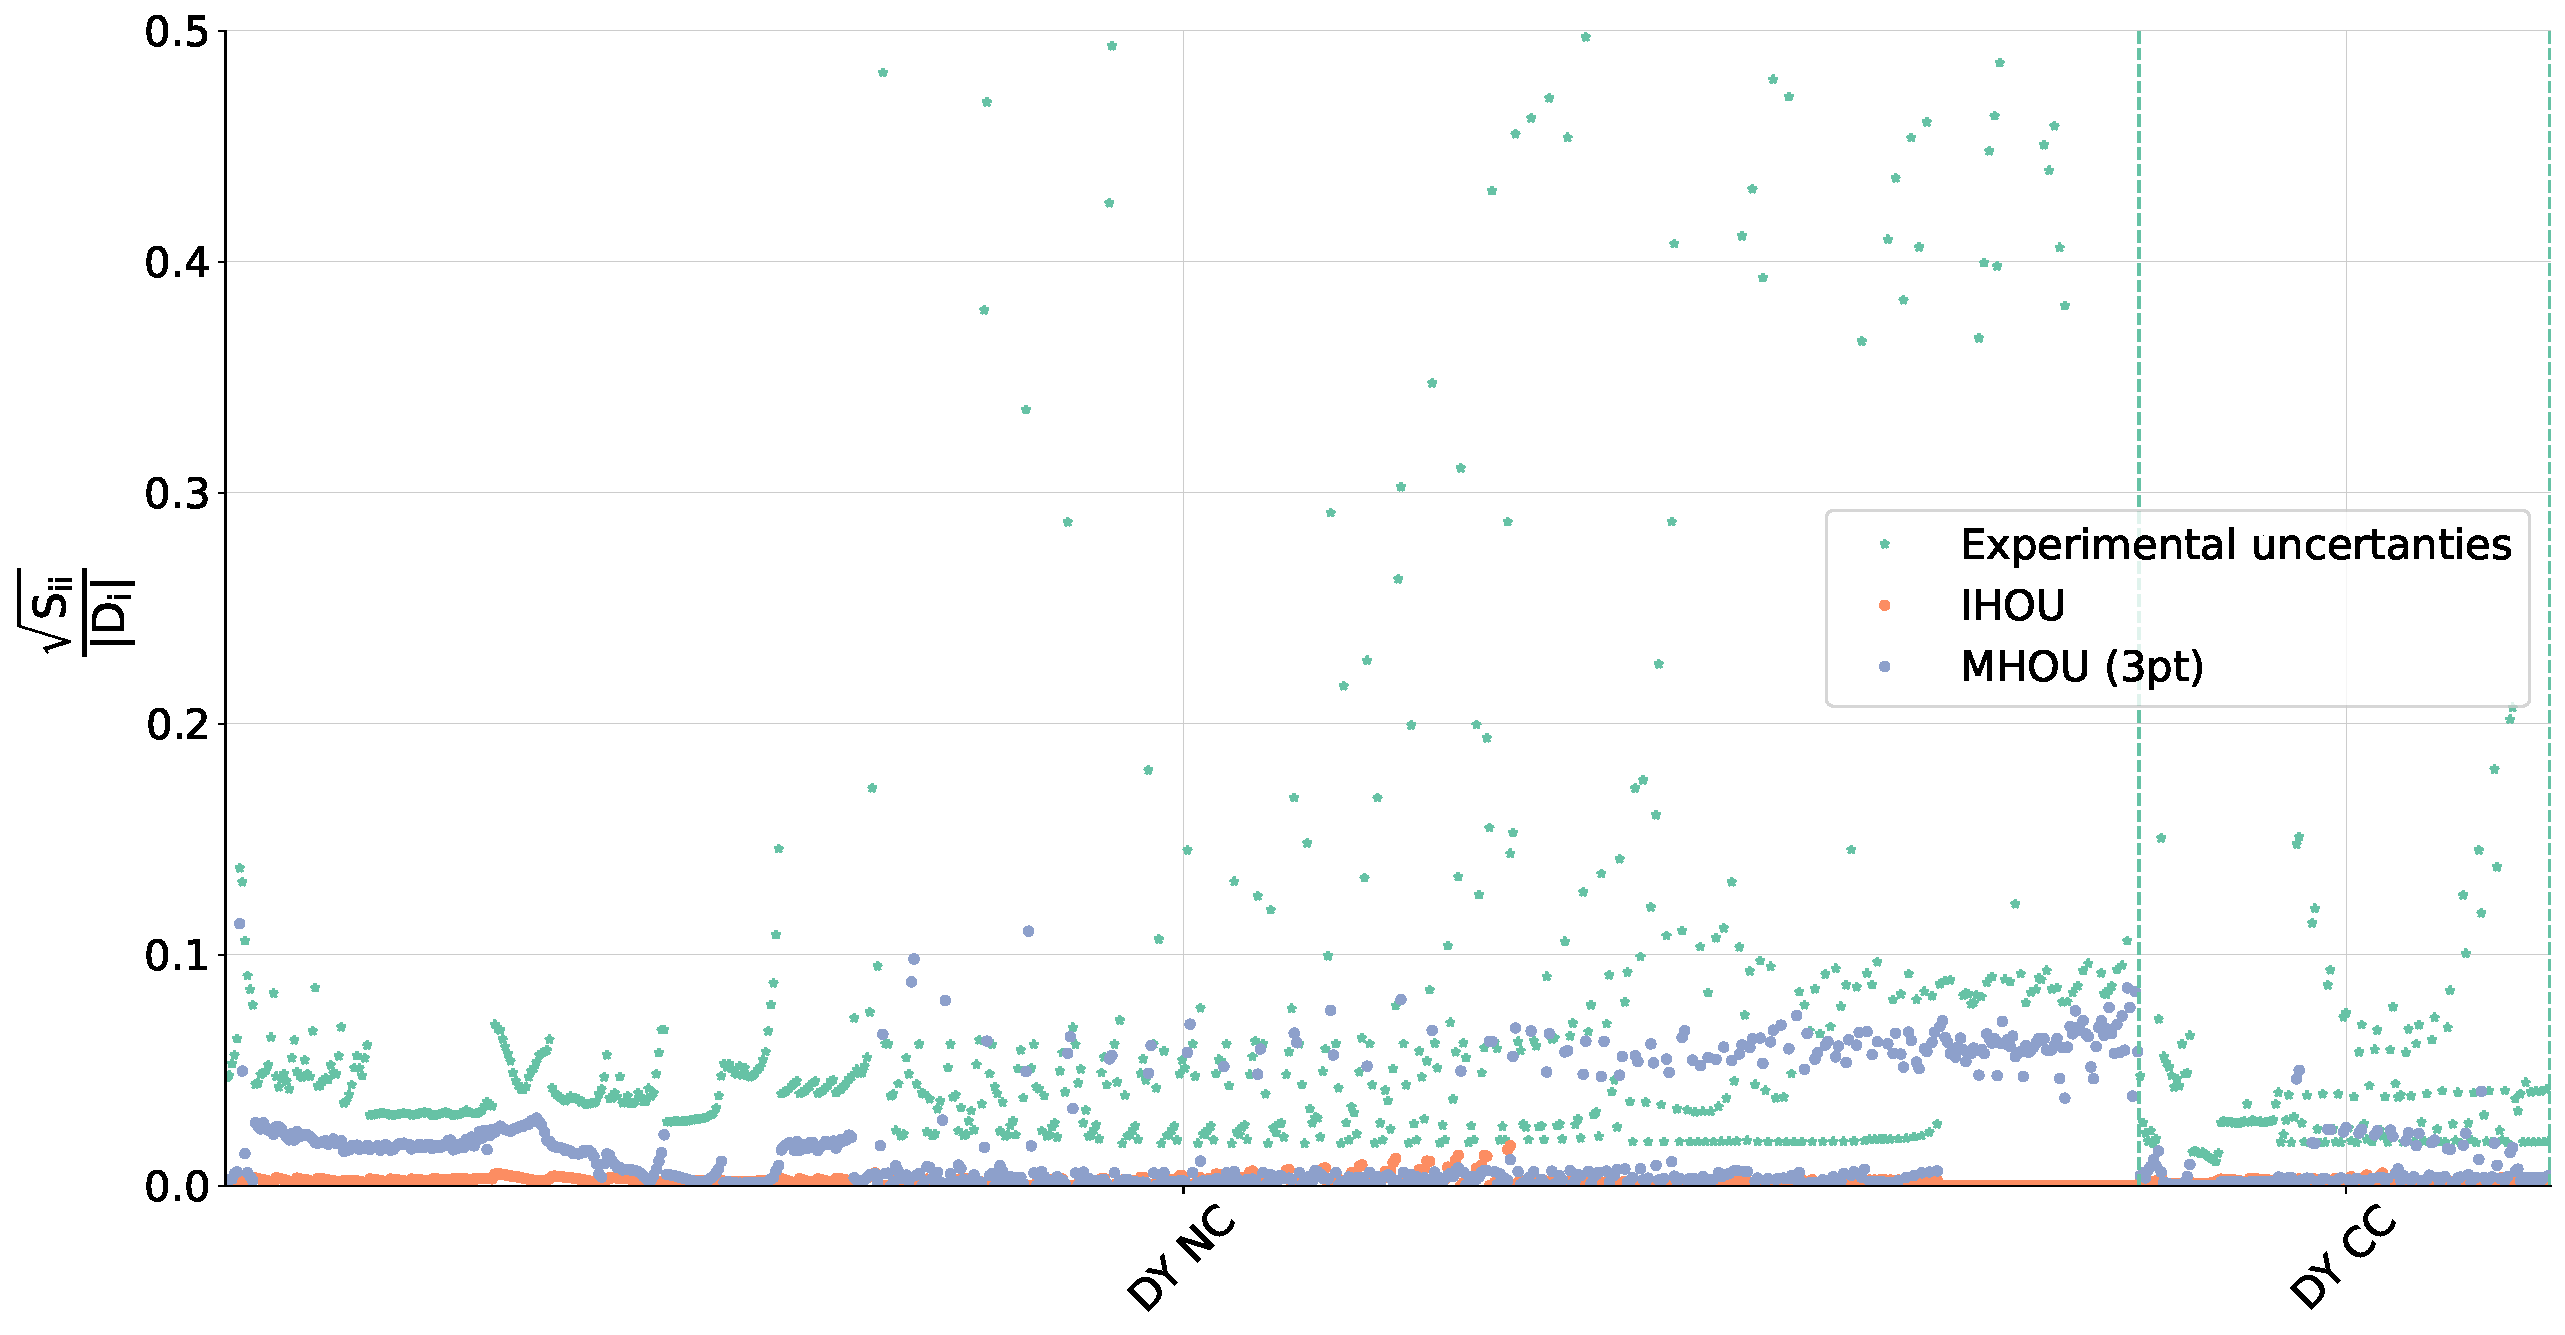
\includegraphics[width=.9\textwidth]{figures/diag_cov_dy_ihou_3pt_mhou.pdf}
        \caption*{NNLO MHOU included where N3LO not available \\
          MHOU can similar magnitude as the experimental uncertainty
        }
      \end{figure}
    \end{column}
  \end{columns}


\end{frame}

% \begin{frame}{Magnitude of theory uncertainties}
% % show that for certain processes th unc is of same size as exp unc.
% \end{frame}

% ============================================================================

\begin{frame}{Impact of MHOUs at N3LO}
  \begin{figure}[!t]
    \centering
    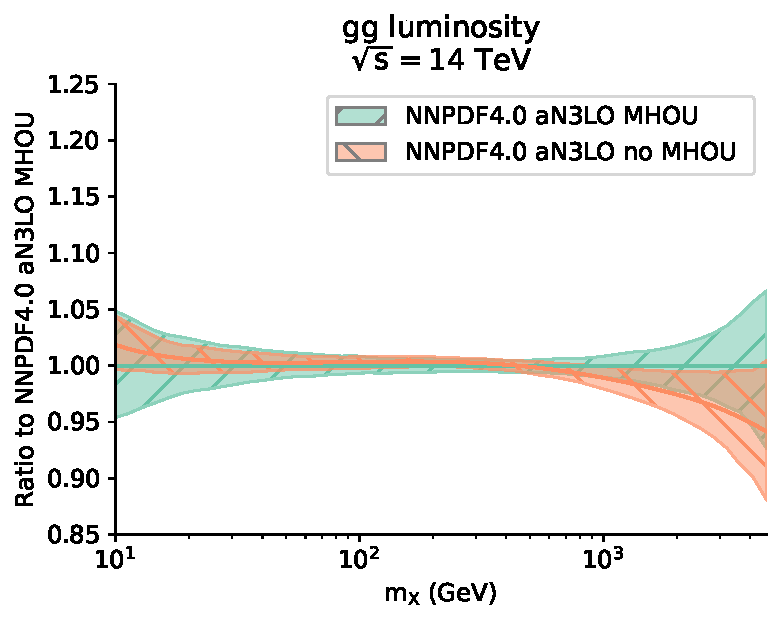
\includegraphics[width=0.45\textwidth]{figures/gg_plot_lumi1d.pdf}
    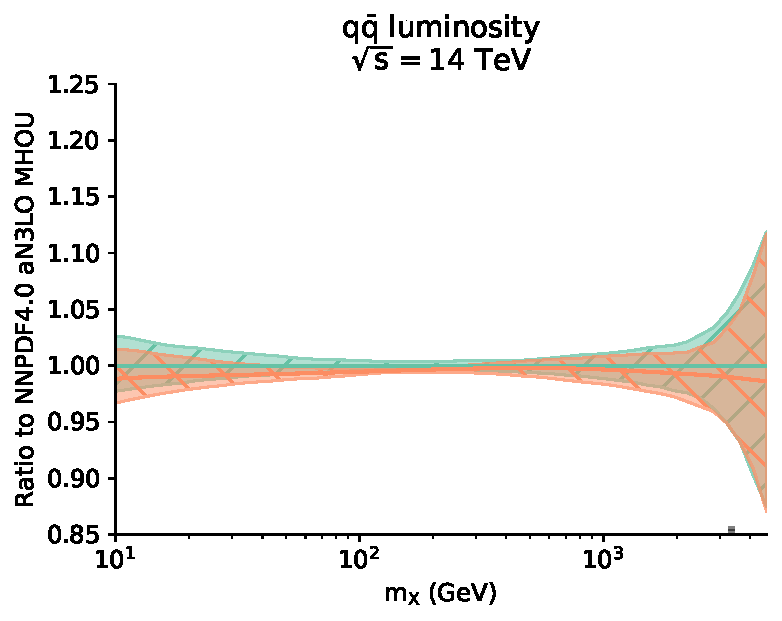
\includegraphics[width=0.45\textwidth]{figures/qqbar_plot_lumi1d.pdf}
  \end{figure}
  \begin{itemize}
    \item Non-negligible impact of MHOUs even at N3LO
    \item[$\Rightarrow$] reason to include exact N3LO calculations for hadronic processes
  \end{itemize}
\end{frame}


% \begin{frame}{Comparison to MSHT20}
%   \begin{figure}[!t]
%     \centering
%     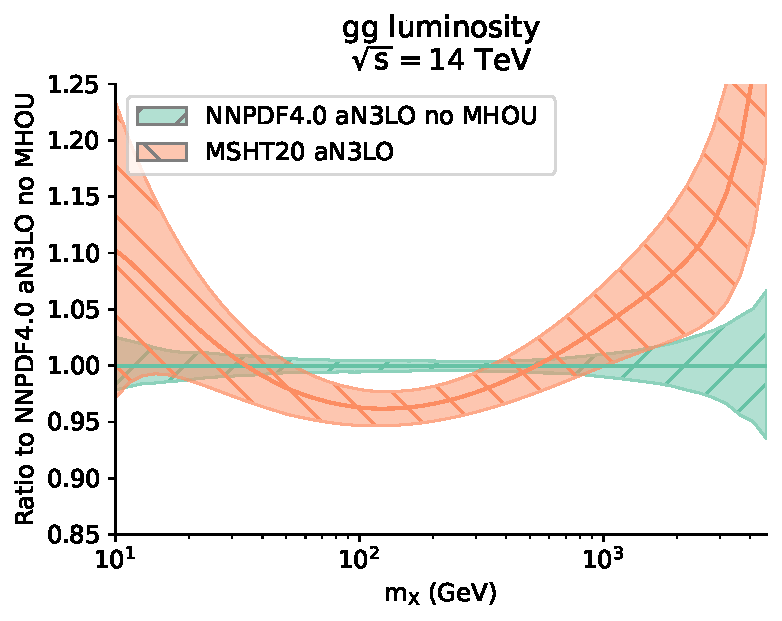
\includegraphics[width=0.45\textwidth]{figures/gg_plot_lumi1d_msht20.pdf}
%     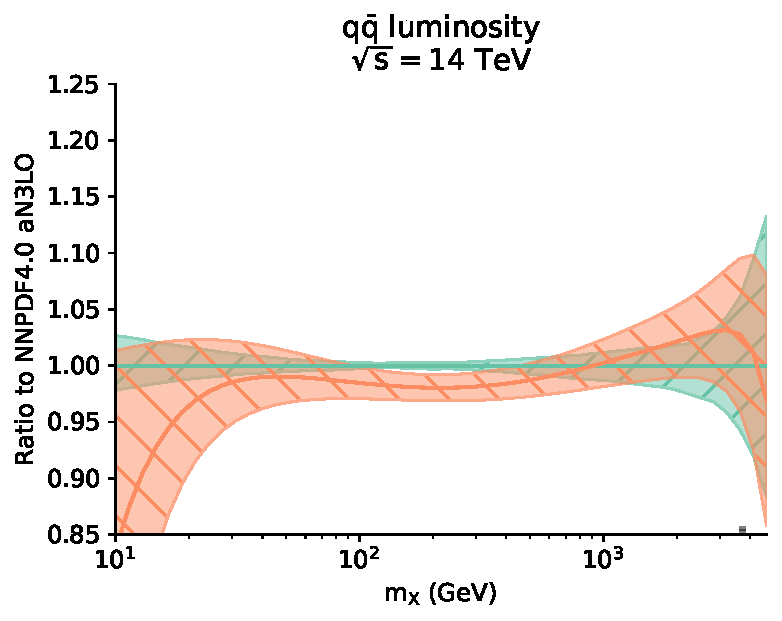
\includegraphics[width=0.45\textwidth]{figures/qqbar_plot_lumi1d_msht20.pdf}
%   \end{figure}
%   \begin{itemize}
%     \item Good agreement with MSHT20 for the quark luminosities
%     \item Also for gluon luminosities, except around the Higgs mass and high-mass
%     \item Similar data but different methodology (including splitting function parametrization)
%   \end{itemize}
% \end{frame}




\end{document}
